\chapter{The Real and Complex Number Systems}
\section{Integers}

\begin{problembox}[1.1: No Largest Prime]
Prove that there is no largest prime. (A proof was known to Euclid.)
\end{problembox}

\textbf{Solution:}
We will prove this by contradiction. Assume there exists a largest prime number, call it $p$.

Consider the number $N = p! + 1$, where $p!$ is the factorial of $p$. 

Since $p!$ is divisible by all integers from $1$ to $p$, the number $N = p! + 1$ is not divisible by any prime number less than or equal to $p$.

Now, $N$ is either prime or composite:
\begin{itemize}
\item If $N$ is prime, then $N > p$, contradicting our assumption that $p$ is the largest prime.
\item If $N$ is composite, then $N$ has a prime factor $q$. Since $N$ is not divisible by any prime $\leq p$, we must have $q > p$. This again contradicts our assumption that $p$ is the largest prime.
\end{itemize}

In both cases, we reach a contradiction. Therefore, our assumption that there exists a largest prime is false, and there must be infinitely many prime numbers.

\begin{problembox}[1.2: Algebraic Identity]
If $n$ is a positive integer, prove the algebraic identity:
\[
a^n - b^n = (a - b)\sum_{k=0}^{n-1} a^k b^{n-1-k}
\]
\end{problembox}

\textbf{Solution:}
We can prove this identity by expanding the right-hand side and showing it equals the left-hand side.

Let's expand the sum:
\begin{align*}
(a - b)\sum_{k=0}^{n-1} a^k b^{n-1-k} &= (a - b)(a^0 b^{n-1} + a^1 b^{n-2} + a^2 b^{n-3} + \cdots + a^{n-1} b^0) \\
&= (a - b)(b^{n-1} + a b^{n-2} + a^2 b^{n-3} + \cdots + a^{n-1})
\end{align*}

Now distribute $(a - b)$:
\begin{align*}
&= a \cdot b^{n-1} + a^2 b^{n-2} + a^3 b^{n-3} + \cdots + a^n \\
&\quad - b \cdot b^{n-1} - a b^{n-1} - a^2 b^{n-2} - \cdots - a^{n-1} b
\end{align*}

Notice that most terms cancel out:
\begin{align*}
&= a^n - b^n + \text{(canceling terms)} \\
&= a^n - b^n
\end{align*}

Alternatively, we can use the geometric series formula. Let $r = \frac{a}{b}$. Then:
\begin{align*}
\sum_{k=0}^{n-1} a^k b^{n-1-k} &= b^{n-1} \sum_{k=0}^{n-1} \left(\frac{a}{b}\right)^k \\
&= b^{n-1} \cdot \frac{1 - \left(\frac{a}{b}\right)^n}{1 - \frac{a}{b}} \\
&= b^{n-1} \cdot \frac{b^n - a^n}{b^n(b - a)} \\
&= \frac{a^n - b^n}{a - b}
\end{align*}

Therefore, $(a - b)\sum_{k=0}^{n-1} a^k b^{n-1-k} = a^n - b^n$.

\begin{problembox}[1.3: Mersenne Primes]
If $2^n - 1$ is prime, prove that $n$ is prime. A prime of the form $2^p - 1$, where $p$ is prime, is called a \textit{Mersenne prime}.
\end{problembox}

\textbf{Solution:}
We will prove the contrapositive: if $n$ is composite, then $2^n - 1$ is composite.

Let $n = ab$ where $a, b > 1$ are integers. Then:
\begin{align*}
2^n - 1 &= 2^{ab} - 1 \\
&= (2^a)^b - 1
\end{align*}

Using the identity from Problem 1.2 with $x = 2^a$ and $y = 1$:
\begin{align*}
(2^a)^b - 1 &= (2^a - 1)((2^a)^{b-1} + (2^a)^{b-2} + \cdots + 2^a + 1)
\end{align*}

Since $a > 1$, we have $2^a - 1 > 1$. Also, since $b > 1$, the second factor is greater than 1. Therefore, $2^n - 1$ is the product of two integers greater than 1, making it composite.

This proves that if $2^n - 1$ is prime, then $n$ must be prime.

\begin{problembox}[1.4: Fermat Primes]
If $2^n + 1$ is prime, prove that $n$ is a power of $2$. A prime of the form $2^{2^n} + 1$ is called a \textit{Fermat prime}. Hint: Use Exercise 1.2.
\end{problembox}

\textbf{Solution:}
We will prove the contrapositive: if $n$ is not a power of $2$, then $2^n + 1$ is composite.

If $n$ is not a power of $2$, then $n$ has an odd factor greater than $1$. Let $n = 2^k \cdot m$ where $m > 1$ is odd and $k \geq 0$.

Then:
\begin{align*}
2^n + 1 &= 2^{2^k \cdot m} + 1 \\
&= (2^{2^k})^m + 1
\end{align*}

Since $m$ is odd, we can use the identity from Problem 1.2 with $a = 2^{2^k}$ and $b = -1$:
\begin{align*}
(2^{2^k})^m - (-1)^m &= (2^{2^k} - (-1))((2^{2^k})^{m-1} + (2^{2^k})^{m-2}(-1) + \cdots + (-1)^{m-1})
\end{align*}

Since $m$ is odd, $(-1)^m = -1$, so:
\begin{align*}
(2^{2^k})^m + 1 &= (2^{2^k} + 1)((2^{2^k})^{m-1} - (2^{2^k})^{m-2} + \cdots + 1)
\end{align*}

Since $m > 1$, both factors are greater than $1$, making $2^n + 1$ composite.

Therefore, if $2^n + 1$ is prime, then $n$ must be a power of $2$.

\begin{problembox}[1.5: Fibonacci Numbers Formula]
The Fibonacci numbers $1, 1, 2, 3, 5, 8, 13, \dots$ are defined by the recursion formula $x_{n+1} = x_n + x_{n-1}$, with $x_1 = x_2 = 1$. Prove that $x_n = \frac{a^n - b^n}{a - b}$, where $a$ and $b$ are the roots of the equation $x^2 - x - 1 = 0$.
\end{problembox}

\textbf{Solution:}
First, let's find the roots of the equation $x^2 - x - 1 = 0$:
\begin{align*}
x &= \frac{1 \pm \sqrt{1 + 4}}{2} \\
&= \frac{1 \pm \sqrt{5}}{2}
\end{align*}

So $a = \frac{1 + \sqrt{5}}{2}$ and $b = \frac{1 - \sqrt{5}}{2}$.

We will prove the formula by induction. Let $F_n = \frac{a^n - b^n}{a - b}$.

\textbf{Base cases:}
For $n = 1$: $F_1 = \frac{a - b}{a - b} = 1 = x_1$
For $n = 2$: $F_2 = \frac{a^2 - b^2}{a - b} = \frac{(a - b)(a + b)}{a - b} = a + b = 1 = x_2$

\textbf{Inductive step:}
Assume $F_k = x_k$ for all $k \leq n$. We need to show $F_{n+1} = x_{n+1}$.

Since $a$ and $b$ are roots of $x^2 - x - 1 = 0$, we have $a^2 = a + 1$ and $b^2 = b + 1$.

Therefore:
\begin{align*}
F_{n+1} &= \frac{a^{n+1} - b^{n+1}}{a - b} \\
&= \frac{a \cdot a^n - b \cdot b^n}{a - b} \\
&= \frac{a \cdot a^n - b \cdot b^n + (a^n - a^n)}{a - b} \\
&= \frac{a^n(a - b) + b(a^n - b^n)}{a - b} \\
&= a^n + b \cdot F_n
\end{align*}

Similarly:
\begin{align*}
F_{n+1} &= \frac{a^{n+1} - b^{n+1}}{a - b} \\
&= \frac{a \cdot a^n - b \cdot b^n + (b^n - b^n)}{a - b} \\
&= \frac{b^n(a - b) + a(a^n - b^n)}{a - b} \\
&= b^n + a \cdot F_n
\end{align*}

Adding these two expressions:
\begin{align*}
2F_{n+1} &= a^n + b^n + (a + b)F_n \\
&= a^n + b^n + F_n
\end{align*}

Since $a + b = 1$, we have:
\begin{align*}
F_{n+1} &= \frac{a^n + b^n + F_n}{2} \\
&= \frac{F_n + F_{n-1}}{2} + \frac{a^n + b^n}{2}
\end{align*}

But by the inductive hypothesis, $F_n = x_n$ and $F_{n-1} = x_{n-1}$, and by the Fibonacci recurrence, $x_{n+1} = x_n + x_{n-1}$.

Therefore, $F_{n+1} = x_{n+1}$, completing the induction.

\begin{problembox}[1.6: Well-Ordering Principle]
Prove that every nonempty set of positive integers contains a smallest member. This is called the \textit{well-ordering principle}.
\end{problembox}

\textbf{Solution:}
Prove by induction on the size of the set $S$ of positive integers.

\textbf{Base case:} If $|S| = 1$, $S = \{a\}$, and $a$ is the smallest element.

\textbf{Inductive step:} Assume every set of $k$ positive integers has a smallest element. Let $S$ have $k+1$ elements. Choose $a \in S$, and let $S' = S \setminus \{a\}$. By the inductive hypothesis, $S'$ has a smallest element $b$. The smallest element of $S$ is $\min(a, b)$, which exists since both are positive integers. Thus, $S$ has a smallest element.


\section{Rational and Irrational Numbers}
\begin{problembox}[1.7: Decimal Expansion to Rational]
Find the rational number whose decimal expansion is $0.334444\ldots$.
\end{problembox}

\textbf{Solution:}
We can use an algebraic method to find the equivalent fraction. Let $x$ be the rational number.
$$x = 0.334444\ldots$$
The goal is to manipulate the equation to eliminate the repeating decimal part. The repeating digit '4' begins at the third decimal place.

First, multiply by $100$ to move the non-repeating part to the left of the decimal point:
$$100x = 33.4444\ldots$$
Next, multiply by $1000$ to shift the decimal point past the first repeating digit:
$$1000x = 334.4444\ldots$$
Now, subtract the first equation from the second. This will cancel the infinite repeating tail.
\begin{align*}
1000x &= 334.4444\ldots \\
-\quad 100x &= \phantom{0}33.4444\ldots \\
\hline
900x &= 301
\end{align*}
Finally, solve for $x$:
$$x = \frac{301}{900}$$
Therefore, the rational number is $\frac{301}{900}$.

\begin{problembox}[1.8: Decimal Expansion Ending in Zeroes]
Prove that the decimal expansion of $x$ will end in zeroes (or in nines) if and only if $x$ is a rational number whose denominator is of the form $2^m 5^n$, where $m$ and $n$ are nonnegative integers.
\end{problembox}

\textbf{Solution:}
We need to prove both directions of this statement.

\textbf{Forward direction:} If $x$ is rational with denominator of the form $2^m 5^n$, then its decimal expansion terminates.

Let $x = \frac{p}{q}$ where $q = 2^m 5^n$ for some nonnegative integers $m, n$.

We can write $x = \frac{p}{2^m 5^n} = \frac{p \cdot 2^n 5^m}{2^m 5^n \cdot 2^n 5^m} = \frac{p \cdot 2^n 5^m}{10^{m+n}}$

This shows that $x$ can be written as a fraction with denominator a power of 10, which means its decimal expansion terminates.

\textbf{Reverse direction:} If the decimal expansion of $x$ terminates, then $x$ is rational with denominator of the form $2^m 5^n$.

Let $x$ have a terminating decimal expansion. Then $x$ can be written as $x = \frac{N}{10^k}$ for some integer $N$ and nonnegative integer $k$.

Since $10 = 2 \cdot 5$, we have $10^k = 2^k \cdot 5^k$, which is of the required form.

\textbf{Note about ending in nines:}
If a decimal expansion ends in nines (e.g., $0.999\ldots$), this is equivalent to the next terminating decimal. For example, $0.999\ldots = 1.000\ldots$. This is because $0.999\ldots = \frac{9}{10} + \frac{9}{100} + \frac{9}{1000} + \cdots = \frac{9/10}{1 - 1/10} = 1$.

Therefore, both terminating decimals and those ending in nines correspond to rational numbers with denominators of the form $2^m 5^n$.

\begin{problembox}[1.9: Irrationality of $\sqrt{2} + \sqrt{3}$]
Prove that $\sqrt{2} + \sqrt{3}$ is irrational.
\end{problembox}

\textbf{Solution:}
We will prove this by contradiction. Assume that $\sqrt{2} + \sqrt{3}$ is rational, say $\sqrt{2} + \sqrt{3} = \frac{p}{q}$ where $p, q$ are integers with no common factors.

Then:
\begin{align*}
\sqrt{2} + \sqrt{3} &= \frac{p}{q} \\
(\sqrt{2} + \sqrt{3})^2 &= \left(\frac{p}{q}\right)^2 \\
2 + 2\sqrt{6} + 3 &= \frac{p^2}{q^2} \\
5 + 2\sqrt{6} &= \frac{p^2}{q^2} \\
2\sqrt{6} &= \frac{p^2}{q^2} - 5 \\
\sqrt{6} &= \frac{p^2 - 5q^2}{2q^2}
\end{align*}

This shows that $\sqrt{6}$ is rational, which is a contradiction since $\sqrt{6}$ is irrational.

To see why $\sqrt{6}$ is irrational, suppose $\sqrt{6} = \frac{a}{b}$ where $a, b$ are integers with no common factors. Then:
\begin{align*}
6 &= \frac{a^2}{b^2} \\
6b^2 &= a^2
\end{align*}

This means $a^2$ is divisible by 6, so $a$ must be divisible by 6. Let $a = 6k$. Then:
\begin{align*}
6b^2 &= (6k)^2 = 36k^2 \\
b^2 &= 6k^2
\end{align*}

This means $b^2$ is divisible by 6, so $b$ must also be divisible by 6. But this contradicts our assumption that $a$ and $b$ have no common factors.

Therefore, $\sqrt{6}$ is irrational, and consequently $\sqrt{2} + \sqrt{3}$ is irrational.

\begin{problembox}[1.10: Rational Functions of Irrational Numbers]
If $a, b, c, d$ are rational and if $x$ is irrational, prove that $\frac{ax + b}{cx + d}$ is usually irrational. When do exceptions occur?
\end{problembox}

\textbf{Solution:}
We need to analyze when $\frac{ax + b}{cx + d}$ is rational, given that $x$ is irrational and $a, b, c, d$ are rational.

Let's assume that $\frac{ax + b}{cx + d} = \frac{p}{q}$ where $p, q$ are integers with no common factors.

Then:
\begin{align*}
\frac{ax + b}{cx + d} &= \frac{p}{q} \\
q(ax + b) &= p(cx + d) \\
qax + qb &= pcx + pd \\
(qa - pc)x &= pd - qb
\end{align*}

Since $x$ is irrational and the right-hand side is rational, we must have $qa - pc = 0$ and $pd - qb = 0$.

This gives us:
\begin{align*}
qa &= pc \\
pd &= qb
\end{align*}

From the first equation: $a = \frac{pc}{q}$
From the second equation: $b = \frac{pd}{q}$

Therefore, we have:
\begin{align*}
\frac{a}{c} &= \frac{p}{q} \\
\frac{b}{d} &= \frac{p}{q}
\end{align*}

This means $\frac{a}{c} = \frac{b}{d}$, or equivalently, $ad = bc$.

\textbf{Conclusion:}
The expression $\frac{ax + b}{cx + d}$ is rational if and only if $ad = bc$.

\textbf{Exceptions occur when:}
$ad = bc$, which means the numerator and denominator are proportional, making the fraction rational regardless of the value of $x$.

\textbf{Examples:}
\begin{itemize}
\item If $a = 2, b = 1, c = 4, d = 2$, then $ad = 4 = bc = 4$, so $\frac{2x + 1}{4x + 2} = \frac{1}{2}$ for all $x$.
\item If $a = 1, b = 0, c = 1, d = 0$, then $ad = 0 = bc = 0$, so $\frac{x}{x} = 1$ for all $x \neq 0$.
\end{itemize}

\begin{problembox}[1.11: Irrational Numbers Between 0 and x]
Given any real $x > 0$, prove that there is an irrational number between $0$ and $x$.
\end{problembox}

\textbf{Solution:}
We will construct an irrational number between $0$ and $x$ for any positive real number $x$.

\textbf{Case 1:} If $x$ is irrational, then $\frac{x}{2}$ is irrational and lies between $0$ and $x$.

To see why $\frac{x}{2}$ is irrational, suppose it were rational. Then $\frac{x}{2} = \frac{p}{q}$ for some integers $p, q$, which would mean $x = \frac{2p}{q}$, making $x$ rational, a contradiction.

\textbf{Case 2:} If $x$ is rational, let $x = \frac{p}{q}$ where $p, q$ are positive integers.

Consider the number $y = \frac{x}{\sqrt{2}} = \frac{p}{q\sqrt{2}}$.

Since $\sqrt{2}$ is irrational, $y$ is irrational (if $y$ were rational, then $\sqrt{2} = \frac{p}{qy}$ would be rational, a contradiction).

Also, since $\sqrt{2} > 1$, we have $y < x$.

Therefore, $y$ is an irrational number between $0$ and $x$.

\textbf{Alternative construction:}
For any positive real $x$, we can also use $y = \frac{x}{\pi}$. Since $\pi$ is irrational and greater than $1$, we have $0 < y < x$, and $y$ is irrational.

\begin{problembox}[1.12: Fraction Between Two Fractions]
If $\frac{a}{b} < \frac{c}{d}$ with $b > 0, d > 0$, prove that $\frac{a + c}{b + d}$ lies between $\frac{a}{b}$ and $\frac{c}{d}$.
\end{problembox}

\textbf{Solution:}
We need to prove that $\frac{a}{b} < \frac{a + c}{b + d} < \frac{c}{d}$.

Let's prove both inequalities:

\textbf{First inequality:} $\frac{a}{b} < \frac{a + c}{b + d}$

Cross-multiplying:
\begin{align*}
a(b + d) &< b(a + c) \\
ab + ad &< ab + bc \\
ad &< bc
\end{align*}

Since $\frac{a}{b} < \frac{c}{d}$, we have $ad < bc$, so this inequality holds.

\textbf{Second inequality:} $\frac{a + c}{b + d} < \frac{c}{d}$

Cross-multiplying:
\begin{align*}
d(a + c) &< c(b + d) \\
ad + cd &< bc + cd \\
ad &< bc
\end{align*}

Again, since $\frac{a}{b} < \frac{c}{d}$, we have $ad < bc$, so this inequality also holds.

Therefore, $\frac{a + c}{b + d}$ lies between $\frac{a}{b}$ and $\frac{c}{d}$.

\textbf{Geometric interpretation:}
This result is known as the "mediant" of two fractions. If we think of fractions as points on a line, the mediant $\frac{a + c}{b + d}$ lies between the two original fractions $\frac{a}{b}$ and $\frac{c}{d}$.

\begin{problembox}[1.13: $\sqrt{2}$ Between Fractions]
Let $a$ and $b$ be positive integers. Prove that $\sqrt{2}$ always lies between the two fractions $\frac{a}{b}$ and $\frac{a + 2b}{a + b}$. Which fraction is closer to $\sqrt{2}$?
\end{problembox}

\textbf{Solution:}
Let's first establish the ordering of the two fractions by examining their difference:
\[
\frac{a + 2b}{a + b} - \frac{a}{b} = \frac{b(a + 2b) - a(a + b)}{b(a + b)} = \frac{ab + 2b^2 - a^2 - ab}{b(a + b)} = \frac{2b^2 - a^2}{b(a + b)}
\]
The sign of this difference depends on the sign of $2b^2 - a^2$, which relates $\frac{a}{b}$ to $\sqrt{2}$.

\textbf{Case 1: $\frac{a}{b} < \sqrt{2}$}. This means $a < b\sqrt{2}$, so $a^2 < 2b^2$, and $2b^2 - a^2 > 0$.
Thus, $\frac{a}{b} < \frac{a+2b}{a+b}$. We need to show that $\frac{a+2b}{a+b} > \sqrt{2}$.
\[
\frac{a + 2b}{a + b} > \sqrt{2} \iff a + 2b > \sqrt{2}(a + b) \iff b(2 - \sqrt{2}) > a(\sqrt{2} - 1) \iff \frac{2 - \sqrt{2}}{\sqrt{2} - 1} > \frac{a}{b}
\]
Since $\frac{2 - \sqrt{2}}{\sqrt{2} - 1} = \frac{\sqrt{2}(\sqrt{2} - 1)}{\sqrt{2} - 1} = \sqrt{2}$, this simplifies to $\sqrt{2} > \frac{a}{b}$, which is true by our case assumption. Thus, $\frac{a}{b} < \sqrt{2} < \frac{a + 2b}{a + b}$.

\textbf{Case 2: $\frac{a}{b} > \sqrt{2}$}. This means $a^2 > 2b^2$, and $2b^2 - a^2 < 0$.
Thus, $\frac{a}{b} > \frac{a+2b}{a+b}$. A similar calculation shows that $\frac{a+2b}{a+b} < \sqrt{2}$.
Therefore, $\frac{a+2b}{a+b} < \sqrt{2} < \frac{a}{b}$. In both cases, $\sqrt{2}$ lies between the two fractions.

\textbf{Which fraction is closer to $\sqrt{2}$?}
We compare the absolute distances:
\begin{itemize}
\item Distance 1: $\left|\frac{a}{b} - \sqrt{2}\right| = \frac{|a - b\sqrt{2}|}{b}$
\item Distance 2: $\left|\frac{a + 2b}{a + b} - \sqrt{2}\right| = \left|\frac{a + 2b - a\sqrt{2} - b\sqrt{2}}{a + b}\right| = \left|\frac{a(1-\sqrt{2}) - b(\sqrt{2}-2)}{a + b}\right| = \frac{|a - b\sqrt{2}|(\sqrt{2}-1)}{a+b}$
\end{itemize}
To see which distance is smaller, we compare $\frac{1}{b}$ with $\frac{\sqrt{2}-1}{a+b}$.
This is equivalent to comparing $a+b$ with $b(\sqrt{2}-1) = b\sqrt{2} - b$, which is equivalent to comparing $a+2b$ with $b\sqrt{2}$, or $\frac{a}{b} + 2$ with $\sqrt{2}$.
Since $a, b$ are positive integers, $\frac{a}{b} > 0$, so $\frac{a}{b} + 2 > 2 > \sqrt{2}$.
This implies $\frac{1}{b} > \frac{\sqrt{2}-1}{a+b}$.
Therefore, Distance 1 is always greater than Distance 2. The new fraction $\frac{a+2b}{a+b}$ is \textbf{always} closer to $\sqrt{2}$.

\section{Inequalities}

\begin{problembox}[1.14: Irrationality of $\sqrt{n - 1} + \sqrt{n + 1}$]
Prove that $\sqrt{n - 1} + \sqrt{n + 1}$ is irrational for every integer $n \geq 1$.
\end{problembox}

\textbf{Solution:}
Assume $\sqrt{n - 1} + \sqrt{n + 1} = \frac{p}{q}$, where $p, q$ are integers, $q \neq 0$, $\gcd(p, q) = 1$.

Square both sides:
\[
(n - 1) + 2\sqrt{(n - 1)(n + 1)} + (n + 1) = \frac{p^2}{q^2} \implies 2n + 2\sqrt{n^2 - 1} = \frac{p^2}{q^2}.
\]
Thus:
\[
\sqrt{n^2 - 1} = \frac{p^2 - 2n q^2}{2 q^2}.
\]
Suppose $\sqrt{n^2 - 1}$ is rational, say $\frac{a}{b}$, $\gcd(a, b) = 1$. Then:
\[
n^2 - 1 = \frac{a^2}{b^2} \implies a^2 = (n^2 - 1)b^2.
\]
For $n = 1$, $\sqrt{0} + \sqrt{2} = \sqrt{2}$, irrational. For $n \geq 2$, $n^2 - 1 = (n - 1)(n + 1)$ is not a perfect square (since $(n - 1)^2 < n^2 - 1 < n^2$). If $a^2 = (n^2 - 1)b^2$, $n^2 - 1$ must be a perfect square, a contradiction for $n \geq 2$. Thus, $\sqrt{n^2 - 1}$ is irrational, so $\sqrt{n - 1} + \sqrt{n + 1}$ is irrational.

\begin{problembox}[1.15: Approximation by Rational Numbers]
Given a real $x$ and an integer $N > 1$, prove that there exist integers $h$ and $k$ with $0 < k \leq N$ such that $|kx - h| < 1/N$. Hint. Consider the $N+1$ numbers $tx-[tx]$ for $t=0,1,2,\dots,N$ and show that some pair differs by at most $1/N$.
\end{problembox}

\textbf{Solution:}
We will use the pigeonhole principle to prove this result.

Consider the $N + 1$ numbers: $0, x, 2x, 3x, \ldots, Nx$.

Let's look at the fractional parts of these numbers. The fractional part of a number $y$ is $y - \lfloor y \rfloor$, where $\lfloor y \rfloor$ is the greatest integer less than or equal to $y$.

The fractional parts of $0, x, 2x, \ldots, Nx$ all lie in the interval $[0, 1)$.

Divide the interval $[0, 1)$ into $N$ equal subintervals:
$[0, 1/N), [1/N, 2/N), \ldots, [(N-1)/N, 1)$

By the pigeonhole principle, since we have $N + 1$ numbers and only $N$ subintervals, at least two of these numbers must fall into the same subinterval.

Let's say $ix$ and $jx$ (where $0 \leq i < j \leq N$) have fractional parts in the same subinterval. Then:
\begin{align*}
|(jx - \lfloor jx \rfloor) - (ix - \lfloor ix \rfloor)| &< \frac{1}{N} \\
|(j - i)x - (\lfloor jx \rfloor - \lfloor ix \rfloor)| &< \frac{1}{N}
\end{align*}

Let $k = j - i$ and $h = \lfloor jx \rfloor - \lfloor ix \rfloor$. Then:
\begin{align*}
|kx - h| &< \frac{1}{N}
\end{align*}

Since $0 < i < j \leq N$, we have $0 < k \leq N$, and $h$ is an integer.

Therefore, we have found integers $h$ and $k$ with $0 < k \leq N$ such that $|kx - h| < 1/N$.

\textbf{Example:}
If $x = \pi$ and $N = 5$, we might find that $3\pi \approx 9.4248$ and $5\pi \approx 15.7080$ have fractional parts in the same subinterval, giving us $|2\pi - 6| < 1/5$.

\begin{problembox}[1.16: Infinitely Many Rational Approximations]
If $x$ is irrational, prove that there are infinitely many rational numbers $h/k$ with $k > 0$ such that $|x - h/k| < 1/k^2$.
\end{problembox}
\textbf{Solution:}
We will construct an infinite sequence of distinct rational numbers satisfying the condition.

From Problem 1.15 (Dirichlet's Approximation Theorem), for any integer $N > 1$, there exist integers $h$ and $k$ with $0 < k \leq N$ such that $|kx - h| < 1/N$.
Dividing by $k$, we get:
\[
\left|x - \frac{h}{k}\right| < \frac{1}{Nk}
\]
Since $k \leq N$, we have $\frac{1}{N} \leq \frac{1}{k}$, which implies $\frac{1}{Nk} \leq \frac{1}{k^2}$.
Thus, for any integer $N>1$, we can find a rational number $h/k$ such that:
\[
\left|x - \frac{h}{k}\right| < \frac{1}{k^2}
\]
Now we must show that this process can generate infinitely many distinct fractions.
Assume, for the sake of contradiction, that there are only a finite number of such rational approximations, say $\{h_1/k_1, h_2/k_2, \ldots, h_m/k_m\}$.
Since $x$ is irrational, for any rational number $h_i/k_i$, the distance $|x - h_i/k_i|$ is non-zero. Let $\epsilon$ be the smallest of these non-zero distances:
\[
\epsilon = \min_{i=1,\dots,m} \left|x - \frac{h_i}{k_i}\right| > 0.
\]
Now, choose an integer $N$ large enough such that $1/N < \epsilon$.
By the result from Problem 1.15, there exist integers $h'$ and $k'$ with $0 < k' \leq N$ such that:
\[
|k'x - h'| < \frac{1}{N}
\]
This implies $|x - h'/k'| < \frac{1}{Nk'} \leq \frac{1}{N}$.
So we have found a new rational approximation $h'/k'$ such that:
\[
\left|x - \frac{h'}{k'}\right| < \frac{1}{N} < \epsilon
\]
Since the approximation error of $h'/k'$ is smaller than $\epsilon$, $h'/k'$ cannot be one of the fractions in our finite list $\{h_1/k_1, \ldots, h_m/k_m\}$. This contradicts our assumption that we had a complete list of all such approximations.
Therefore, there must be infinitely many such rational numbers.


\begin{problembox}[1.17: Factorial Representation of Rationals (Precise Form)]
Let $x$ be a positive rational number of the form
\[
x = \sum_{k=1}^n \frac{a_k}{k!},
\]
where each $a_k$ is a nonnegative integer with $a_k \leq k - 1$ for $k \geq 2$ and $a_n > 0$. Let $[x]$ denote the greatest integer less than or equal to $x$. Prove that $a_1 = [x]$, that
\[
a_k = [k!x] - k[(k - 1)!x] \quad \text{for } k = 2, \dots, n,
\]
and that $n$ is the smallest integer such that $n!x$ is an integer. Conversely, show that every positive rational number $x$ can be expressed in this form in one and only one way.
\end{problembox}

\textbf{Solution:}
Let $x = \sum_{k=1}^n \frac{a_k}{k!}$ with the given conditions on $a_k$.

\textbf{1. Proof that $a_1 = [x]$:}
The sum can be written as $x = a_1 + \sum_{k=2}^n \frac{a_k}{k!}$. We must show the summation part is a positive fraction less than 1. Since $a_n > 0$, the sum is positive. We can bound the sum using the property $a_k \leq k-1$:
\[
\sum_{k=2}^n \frac{a_k}{k!} \leq \sum_{k=2}^n \frac{k-1}{k!} < \sum_{k=2}^{\infty} \frac{k-1}{k!}
\]
The infinite sum is a known identity: $\sum_{k=2}^{\infty} \frac{k-1}{k!} = \sum_{k=2}^{\infty} \left(\frac{1}{(k-1)!} - \frac{1}{k!}\right)$. This is a telescoping series whose sum is the first term, $1/(2-1)! = 1$.
Thus, $0 < \sum_{k=2}^n \frac{a_k}{k!} < 1$. This means $a_1 < x < a_1 + 1$, so by definition, $a_1 = [x]$.

\textbf{2. Formula for $a_k$:}
Define $x_1 = x - a_1 = \sum_{k=2}^n \frac{a_k}{k!}$. Then $k!x_1$ is an integer for $k \ge n$.
Consider the expression $k!x - k((k-1)!x) = k!(a_1+x_1) - k((k-1)!(a_1+x_1)) = ka_1k!/k! ...$ this gets complicated.
Let's use the given formula. Let $x_k = k!x - \sum_{j=1}^{k} a_j \frac{k!}{j!} = \sum_{j=k+1}^{n} a_j \frac{k!}{j!} = \frac{a_{k+1}}{k+1} + \frac{a_{k+2}}{(k+1)(k+2)} + \dots$.
From part (1), we know $0 \le x_k < 1$. So $[k!x] = \sum_{j=1}^{k} a_j \frac{k!}{j!}$.
Let's test the formula: $a_k = [k!x] - k[(k - 1)!x]$.
We have $[k!x] = k! \sum_{j=1}^k \frac{a_j}{j!}$ and $[(k-1)!x] = (k-1)! \sum_{j=1}^{k-1} \frac{a_j}{j!}$.
So, $[k!x] - k[(k-1)!x] = \sum_{j=1}^k a_j \frac{k!}{j!} - k \sum_{j=1}^{k-1} a_j \frac{(k-1)!}{j!} = \left(a_k + k\sum_{j=1}^{k-1} a_j \frac{(k-1)!}{j!}\right) - k\sum_{j=1}^{k-1} a_j \frac{(k-1)!}{j!} = a_k$.
This proves the formula for $a_k$.

\textbf{3. Minimality of $n$:}
Multiplying $x$ by $n!$ gives $n!x = \sum_{k=1}^n a_k \frac{n!}{k!}$. Since $k \le n$, each term $\frac{n!}{k!}$ is an integer, so $n!x$ is an integer.
For any $m < n$, when we compute $m!x$, the term corresponding to $k=n$ is $m! \frac{a_n}{n!} = \frac{a_n}{n(n-1)\dots(m+1)}$. Since $0 < a_n \le n-1$, this term is a non-integer fraction. Because all other terms for $k>m$ are also fractions and terms for $k\le m$ are integers, $m!x$ cannot be an integer. Thus, $n$ is the smallest such integer.

\textbf{4. Converse (Existence and Uniqueness):}
\textit{Existence:} Let $x$ be any positive rational. Let $n$ be the smallest integer so $n!x$ is an integer. Define the coefficients $a_k$ recursively:
$a_1 = [x]$, and $x_1 = x - a_1$.
$a_2 = [2!x_1]$, and $x_2 = 2!x_1 - a_2$.
In general, define $x_{k-1}$ for $k \ge 2$. Let $a_k = [k!x_{k-1}]$ and $x_k = k!x_{k-1} - a_k$.
One can prove by induction that $0 \le x_k < 1$ and $a_k \le k-1$ for $k \ge 2$. The process terminates with $x_n=0$ because $n!x$ is an integer.
\textit{Uniqueness:} Suppose $x$ has two different representations, $\sum \frac{a_k}{k!} = \sum \frac{b_k}{k!}$. Let $j$ be the largest index where $a_j \neq b_j$. Assume $a_j > b_j$. Then $\frac{a_j - b_j}{j!} = \sum_{k=1}^{j-1} \frac{b_k - a_k}{k!}$. The left side is $\ge 1/j!$. The right side is bounded above by $\sum_{k=1}^{j-1} \frac{k-1}{k!} < 1/j!$, a contradiction. Thus, all coefficients must be the same.


\section{Upper Bounds}

\begin{problembox}[1.18: Uniqueness of Supremum and Infimum]
Show that the $\sup$ and $\inf$ of a set are uniquely determined whenever they exist.
\end{problembox}

\textbf{Solution:}
We will prove that if a set has a supremum, it is unique. The proof for infimum is similar.

\textbf{Proof by contradiction:}
Suppose a set $S$ has two different suprema, say $s_1$ and $s_2$, with $s_1 < s_2$.

Since $s_1$ is a supremum of $S$:
1. $s_1$ is an upper bound of $S$ (every element of $S$ is $\leq s_1$)
2. $s_1$ is the least upper bound (no number less than $s_1$ is an upper bound)

Since $s_2$ is also a supremum of $S$:
1. $s_2$ is an upper bound of $S$ (every element of $S$ is $\leq s_2$)
2. $s_2$ is the least upper bound (no number less than $s_2$ is an upper bound)

But since $s_1 < s_2$, the number $s_1$ is less than $s_2$ and is also an upper bound of $S$. This contradicts the fact that $s_2$ is the least upper bound.

Therefore, our assumption that there are two different suprema is false, and the supremum must be unique.

\textbf{Alternative proof:}
Let $s_1$ and $s_2$ both be suprema of $S$. Then:
- $s_1$ is an upper bound, so $s_2 \leq s_1$ (since $s_2$ is the least upper bound)
- $s_2$ is an upper bound, so $s_1 \leq s_2$ (since $s_1$ is the least upper bound)

Therefore, $s_1 = s_2$.

\textbf{For infimum:}
The same argument applies to infimum. If a set has two infima $i_1$ and $i_2$, then:
- $i_1$ is a lower bound, so $i_1 \leq i_2$ (since $i_1$ is the greatest lower bound)
- $i_2$ is a lower bound, so $i_2 \leq i_1$ (since $i_2$ is the greatest lower bound)

Therefore, $i_1 = i_2$.

\begin{problembox}[1.19: Finding Supremum and Infimum]
Find the $\sup$ and $\inf$ of each of the following sets:
\begin{enumerate}[label=(\alph*)]
\item All numbers of the form $2^{-p} + 3^{-q} + 5^{-r}$ for positive integers $p, q, r$.
\item $S = \{x : 3x^2 - 10x + 3 < 0\}$.
\item $S = \{x : (x - a)(x - b)(x - c)(x - d) < 0\}$ where $a < b < c < d$.
\end{enumerate}
\end{problembox}

\textbf{Solution:}

\textbf{1. Numbers of the form $2^{-p} + 3^{-q} + 5^{-r}$:}

Let's analyze the range of each term:
- $2^{-p}$ ranges from $\frac{1}{2}$ (when $p = 1$) to $0$ (as $p \to \infty$)
- $3^{-q}$ ranges from $\frac{1}{3}$ (when $q = 1$) to $0$ (as $q \to \infty$)
- $5^{-r}$ ranges from $\frac{1}{5}$ (when $r = 1$) to $0$ (as $r \to \infty$)

Therefore:
- The maximum value occurs when $p = q = r = 1$: $\frac{1}{2} + \frac{1}{3} + \frac{1}{5} = \frac{15 + 10 + 6}{30} = \frac{31}{30}$
- The minimum value occurs as $p, q, r \to \infty$: $0 + 0 + 0 = 0$

So $\sup = \frac{31}{30}$ and $\inf = 0$.

\textbf{2. Set $S = \{x : 3x^2 - 10x + 3 < 0\}$:}

First, let's find the roots of $3x^2 - 10x + 3 = 0$:
\begin{align*}
x &= \frac{10 \pm \sqrt{100 - 36}}{6} \\
&= \frac{10 \pm \sqrt{64}}{6} \\
&= \frac{10 \pm 8}{6} \\
&= \frac{18}{6} = 3 \quad \text{or} \quad \frac{2}{6} = \frac{1}{3}
\end{align*}

Since the coefficient of $x^2$ is positive, the parabola opens upward. The inequality $3x^2 - 10x + 3 < 0$ holds between the roots.

Therefore, $S = (\frac{1}{3}, 3)$, so $\sup = 3$ and $\inf = \frac{1}{3}$.

\textbf{3. Set $S = \{x : (x - a)(x - b)(x - c)(x - d) < 0\}$ where $a < b < c < d$:}

The expression $(x - a)(x - b)(x - c)(x - d)$ changes sign at each root $a, b, c, d$.

Starting from $-\infty$:
- For $x < a$: all factors are negative, so the product is positive
- For $a < x < b$: one factor is positive, three negative, so product is negative
- For $b < x < c$: two factors positive, two negative, so product is positive
- For $c < x < d$: three factors positive, one negative, so product is negative
- For $x > d$: all factors are positive, so product is positive

Therefore, $S = (a, b) \cup (c, d)$.

So $\sup = d$ and $\inf = a$.

\begin{problembox}[1.20: Comparison Property for Suprema]
Let \( S \) and \( T \) be nonempty subsets of \( \mathbb{R} \) such that \( s \leq t \) for all \( s \in S \) and \( t \in T \). Suppose \( T \) has a supremum. Then \( S \) has a supremum and
\[
\sup S \leq \sup T.
\]
\end{problembox}

\textbf{Solution:}
Let $S$ and $T$ be nonempty subsets of $\mathbb{R}$ with the property that for every $s \in S$ and $t \in T$, we have $s \leq t$.

1.  \textbf{Existence of $\sup S$}:
Since $T$ is nonempty, we can pick an arbitrary element $t_0 \in T$. By the given property, for every $s \in S$, we have $s \leq t_0$. This shows that $S$ is bounded above (by any element of $T$). Since $S$ is also nonempty and bounded above, the completeness axiom of $\mathbb{R}$ guarantees that $\sup S$ exists. Let's call it $\alpha = \sup S$.

2.  \textbf{Proof that $\sup S \leq \sup T$}:
Let $\alpha = \sup S$ and $\beta = \sup T$.
From step 1, we know that any element $t \in T$ is an upper bound for the set $S$.
Since $\alpha$ is the *least* upper bound of $S$, it must be less than or equal to any other upper bound of $S$. Therefore, for any $t \in T$, we must have:
\[
\alpha \leq t
\]
This inequality shows that $\alpha$ is a lower bound for the set $T$.
Now, by definition, $\beta = \sup T$ is the least upper bound of $T$. As an upper bound for $T$, $\beta$ must be greater than or equal to every element of $T$. More importantly, it must be greater than or equal to any *lower bound* of $T$.
Since we have established that $\alpha$ is a lower bound for $T$, it must follow that:
\[
\alpha \leq \beta
\]
Substituting the definitions of $\alpha$ and $\beta$, we get:
\[
\sup S \leq \sup T
\]
This completes the proof.

\begin{problembox}[1.21: Product of Suprema]
Let \( A \) and \( B \) be two sets of positive real numbers, each bounded above. Let \( a = \sup A \), \( b = \sup B \). Define
\[
C = \{ xy : x \in A,\, y \in B \}.
\]
Prove that
\[
\sup C = ab.
\]
\end{problembox}

\textbf{Proof:}

Since \( A \) and \( B \) are sets of positive real numbers bounded above, their suprema \( a = \sup A \) and \( b = \sup B \) exist and are finite.

We are to prove that:
\[
\sup C = ab.
\]

\textbf{Step 1: Show that \( ab \) is an upper bound for \( C \).}

Let \( x \in A \), \( y \in B \). Since \( x \leq a \) and \( y \leq b \), we have:
\[
xy \leq ab.
\]
Therefore, every element \( c \in C \) satisfies \( c \leq ab \), so \( ab \) is an upper bound for \( C \).

\textbf{Step 2: Show that \( ab \) is the least upper bound.}

Let \( \varepsilon > 0 \). Since \( a = \sup A \), there exists \( x_\varepsilon \in A \) such that:
\[
x_\varepsilon > a - \frac{\varepsilon}{2b}.
\]
Similarly, since \( b = \sup B \), there exists \( y_\varepsilon \in B \) such that:
\[
y_\varepsilon > b - \frac{\varepsilon}{2a}.
\]

Now consider:
\[
x_\varepsilon y_\varepsilon > \left(a - \frac{\varepsilon}{2b}\right)\left(b - \frac{\varepsilon}{2a}\right) = ab - \frac{\varepsilon}{2} - \frac{\varepsilon}{2} + \frac{\varepsilon^2}{4ab}.
\]
Since \( \frac{\varepsilon^2}{4ab} > 0 \), we have:
\[
x_\varepsilon y_\varepsilon > ab - \varepsilon.
\]
Therefore, for every \( \varepsilon > 0 \), there exists \( c \in C \) such that \( c > ab - \varepsilon \). Hence, \( ab \) is the least upper bound of \( C \).

\[
\boxed{\sup C = ab}
\]

\begin{problembox}[1.22: Representation of Rationals in Base \( k \)]
    Given \( x \geq 0 \) and an integer \( k \geq 2 \), let \( a_0 \) denote the largest integer \( \leq x \), and, assuming that \( a_0, a_1, \dots, a_{n-1} \) have been defined, let \( a_n \) denote the largest integer such that
    \[
    a_0 + \frac{a_1}{k} + \frac{a_2}{k^2} + \cdots + \frac{a_n}{k^n} \leq x.
    \]
    
    \begin{enumerate}
    \item[(a)] Prove that \( 0 \leq a_i \leq k - 1 \) for each \( i = 1, 2, \dots \).
    \item[(b)] Let \( r_n = a_0 + a_1 k^{-1} + a_2 k^{-2} + \cdots + a_n k^{-n} \) and show that \( x = \sup \{ r_n \} \), the supremum of the set of rational numbers \( r_1, r_2, \dots \).
    \end{enumerate}
    \end{problembox}
    
    \textbf{Solution:}
    Let \( r_n = \sum_{i=0}^n \frac{a_i}{k^i} \). By definition, \( a_n \) is the largest integer such that \( r_n \leq x \).
    
    \textbf{(a) Show \( 0 \leq a_i \leq k - 1 \):}
    Since \( a_n \) is the largest integer satisfying the condition, choosing \( a_n + 1 \) would violate it:
    \[
    r_{n-1} + \frac{a_n + 1}{k^n} > x
    \]
    From the definition of \(a_{n-1}\), we know it was the largest integer such that \( r_{n-1} \le x \). This implies $x - r_{n-1} < \frac{1}{k^{n-1}}$.
    Now, from the definition of $a_n$, we have $r_{n-1} + \frac{a_n}{k^n} \leq x$, which implies $a_n \leq k^n(x - r_{n-1})$.
    Combining these facts:
    \[
    a_n \leq k^n(x - r_{n-1}) < k^n\left(\frac{1}{k^{n-1}}\right) = k.
    \]
    Since $a_n$ is an integer and $a_n < k$, we must have $a_n \leq k-1$. Also, $a_n$ must be non-negative, otherwise we could choose $a_n=0$ to get a larger (or equal) sum $r_n$ that is still less than or equal to $x$, contradicting the "largest integer" definition if the original $a_n$ were negative. Thus, $0 \leq a_n \leq k-1$.
    
    \textbf{(b) Show that \( x = \sup \{ r_n \} \):}
    The sequence $\{r_n\}$ is non-decreasing by construction, since $a_n \ge 0$. It is also bounded above by $x$. Therefore, its supremum exists; let $r = \sup\{r_n\}$. We know $r \le x$.
    We will prove $r=x$ by contradiction. Assume $r < x$. Let $\delta = x - r > 0$.
    By the Archimedean property, we can choose an integer $N$ large enough such that $\frac{1}{k^N} < \delta$.
    From the definition of $a_N$, we know $r_N = r_{N-1} + \frac{a_N}{k^N} \le x$ and $r_{N-1} + \frac{a_N+1}{k^N} > x$.
    The second inequality rearranges to $x - r_N < \frac{1}{k^N}$.
    Since $r = \sup\{r_n\}$, we know $r_N \leq r$.
    Therefore, $x - r \leq x - r_N < \frac{1}{k^N}$.
    Substituting $\delta = x-r$, we get $\delta < \frac{1}{k^N}$.
    But we chose $N$ such that $\frac{1}{k^N} < \delta$. This gives $\delta < \frac{1}{k^N} < \delta$, a contradiction.
    Thus, our assumption must be false, and $x = r = \sup\{r_n\}$.

\section{Inequalities and Identities}
\begin{problembox}[1.23: Lagrange's Identity]
    Prove Lagrange’s identity for real numbers:
    \[
    \left( \sum_{k=1}^n a_k b_k \right)^2 = \left( \sum_{k=1}^n a_k^2 \right)\left( \sum_{k=1}^n b_k^2 \right) - \sum_{1 \leq k < j \leq n} (a_k b_j - a_j b_k)^2.
    \]
    \end{problembox}
    
    \textbf{Proof:}
    We will prove the equivalent identity:
    \[
    \left( \sum_{k=1}^n a_k^2 \right)\left( \sum_{k=1}^n b_k^2 \right) = \left( \sum_{k=1}^n a_k b_k \right)^2 + \sum_{1 \leq k < j \leq n} (a_k b_j - a_j b_k)^2.
    \]
    Let's expand the terms. The left-hand side (LHS) is:
    \begin{align*}
    \left( \sum_{k=1}^n a_k^2 \right)\left( \sum_{j=1}^n b_j^2 \right) &= \sum_{k=1}^n \sum_{j=1}^n a_k^2 b_j^2 \\
    &= \sum_{k=j} a_k^2 b_j^2 + \sum_{k \neq j} a_k^2 b_j^2 \\
    &= \sum_{k=1}^n a_k^2 b_k^2 + \sum_{1 \leq k < j \leq n} (a_k^2 b_j^2 + a_j^2 b_k^2)
    \end{align*}
    Now we expand the terms on the right-hand side (RHS). The first term is:
    \begin{align*}
    \left( \sum_{k=1}^n a_k b_k \right)^2 &= \left( \sum_{k=1}^n a_k b_k \right)\left( \sum_{j=1}^n a_j b_j \right) = \sum_{k=1}^n \sum_{j=1}^n a_k b_k a_j b_j \\
    &= \sum_{k=j} a_k b_k a_j b_j + \sum_{k \neq j} a_k b_k a_j b_j \\
    &= \sum_{k=1}^n a_k^2 b_k^2 + 2 \sum_{1 \leq k < j \leq n} a_k b_k a_j b_j
    \end{align*}
    The second term on the RHS is:
    \[
    \sum_{1 \leq k < j \leq n} (a_k b_j - a_j b_k)^2 = \sum_{1 \leq k < j \leq n} (a_k^2 b_j^2 - 2a_k b_j a_j b_k + a_j^2 b_k^2)
    \]
    Adding the two terms on the RHS gives:
    \begin{align*}
    \text{RHS} &= \left( \sum_{k=1}^n a_k^2 b_k^2 + 2 \sum_{1 \leq k < j \leq n} a_k b_k a_j b_j \right) + \left( \sum_{1 \leq k < j \leq n} (a_k^2 b_j^2 - 2a_k a_j b_k b_j + a_j^2 b_k^2) \right) \\
    &= \sum_{k=1}^n a_k^2 b_k^2 + \sum_{1 \leq k < j \leq n} (a_k^2 b_j^2 + a_j^2 b_k^2)
    \end{align*}
    The RHS now matches our expansion of the LHS, which completes the proof.


    \begin{problembox}[1.24: A Holder-type Inequality]
        Prove that for arbitrary real numbers \( a_k, b_k, c_k \) we have
        \[
        \left( \sum_{k=1}^n a_k b_k c_k \right)^4 \leq
        \left( \sum_{k=1}^n a_k^4 \right)
        \left( \sum_{k=1}^n b_k^2 \right)^2
        \left( \sum_{k=1}^n c_k^4 \right).
        \]
        \end{problembox}
        
        \textbf{Proof:}
        We will prove this inequality by applying the Cauchy-Schwarz inequality twice.
        First, group the terms as $(a_k c_k)$ and $b_k$. Applying the Cauchy-Schwarz inequality to the sequences $\{a_k c_k\}$ and $\{b_k\}$ gives:
        \[
        \left( \sum_{k=1}^n (a_k c_k) b_k \right)^2 \leq \left( \sum_{k=1}^n (a_k c_k)^2 \right) \left( \sum_{k=1}^n b_k^2 \right) = \left( \sum_{k=1}^n a_k^2 c_k^2 \right) \left( \sum_{k=1}^n b_k^2 \right).
        \]
        Next, we apply the Cauchy-Schwarz inequality to the term $\sum_{k=1}^n a_k^2 c_k^2$, treating it as the dot product of sequences $\{a_k^2\}$ and $\{c_k^2\}$:
        \[
        \left( \sum_{k=1}^n a_k^2 c_k^2 \right)^2 \leq \left( \sum_{k=1}^n (a_k^2)^2 \right) \left( \sum_{k=1}^n (c_k^2)^2 \right) = \left( \sum_{k=1}^n a_k^4 \right) \left( \sum_{k=1}^n c_k^4 \right).
        \]
        This implies:
        \[
        \sum_{k=1}^n a_k^2 c_k^2 \leq \left( \sum_{k=1}^n a_k^4 \right)^{1/2} \left( \sum_{k=1}^n c_k^4 \right)^{1/2}.
        \]
        Now, substitute this result back into our first inequality:
        \[
        \left( \sum_{k=1}^n a_k b_k c_k \right)^2 \leq \left( \sum_{k=1}^n a_k^4 \right)^{1/2} \left( \sum_{k=1}^n c_k^4 \right)^{1/2} \left( \sum_{k=1}^n b_k^2 \right).
        \]
        Finally, squaring both sides gives the desired result:
        \[
        \left( \sum_{k=1}^n a_k b_k c_k \right)^4 \leq \left( \sum_{k=1}^n a_k^4 \right) \left( \sum_{k=1}^n c_k^4 \right) \left( \sum_{k=1}^n b_k^2 \right)^2.
        \]

\begin{problembox}[1.25: Minkowski's Inequality]
Prove Minkowski’s inequality:
\[
\left( \sum_{k=1}^n (a_k + b_k)^2 \right)^{1/2} \leq \left( \sum_{k=1}^n a_k^2 \right)^{1/2} + \left( \sum_{k=1}^n b_k^2 \right)^{1/2}.
\]
\end{problembox}

\textbf{Proof:}

Let \( A = \left( \sum a_k^2 \right)^{1/2} \), \( B = \left( \sum b_k^2 \right)^{1/2} \), and expand the square:
\[
\sum (a_k + b_k)^2 = \sum a_k^2 + 2\sum a_k b_k + \sum b_k^2 = A^2 + 2\sum a_k b_k + B^2.
\]

Apply Cauchy–Schwarz:
\[
\sum a_k b_k \leq A B.
\]
Thus,
\[
\sum (a_k + b_k)^2 \leq A^2 + 2AB + B^2 = (A + B)^2.
\]
Taking square roots:
\[
\left( \sum (a_k + b_k)^2 \right)^{1/2} \leq A + B.
\]


\begin{problembox}[1.26: Chebyshev's Sum Inequality]
    If \( a_1 \geq a_2 \geq \cdots \geq a_n \) and \( b_1 \geq b_2 \geq \cdots \geq b_n \), prove that
    \[
    \left( \sum_{k=1}^n a_k \right)\left( \sum_{k=1}^n b_k \right) \leq n \sum_{k=1}^n a_k b_k.
    \]
    \end{problembox}
    
    \textbf{Proof:}
    Consider the double summation
    \[ S = \sum_{i=1}^n \sum_{j=1}^n (a_i - a_j)(b_i - b_j). \]
    Since the sequences $\{a_k\}$ and $\{b_k\}$ are sorted in the same order (both non-increasing), the terms $(a_i - a_j)$ and $(b_i - b_j)$ always have the same sign. If $i>j$, then $a_i \le a_j$ and $b_i \le b_j$, so both differences are non-positive. If $i<j$, both are non-negative. Therefore, their product is always non-negative:
    \[ (a_i - a_j)(b_i - b_j) \geq 0. \]
    This implies that the total sum $S$ must be non-negative, $S \geq 0$.
    
    Now, let's expand the sum:
    \begin{align*}
    S &= \sum_{i=1}^n \sum_{j=1}^n (a_i b_i - a_i b_j - a_j b_i + a_j b_j) \\
    &= \sum_{i=1}^n \sum_{j=1}^n a_i b_i - \sum_{i=1}^n \sum_{j=1}^n a_i b_j - \sum_{i=1}^n \sum_{j=1}^n a_j b_i + \sum_{i=1}^n \sum_{j=1}^n a_j b_j
    \end{align*}
    We evaluate each double summation:
    \begin{itemize}
        \item \( \sum_{i=1}^n \sum_{j=1}^n a_i b_i = \sum_{i=1}^n \left( n \cdot a_i b_i \right) = n \sum_{i=1}^n a_i b_i \)
        \item \( \sum_{i=1}^n \sum_{j=1}^n a_i b_j = \left( \sum_{i=1}^n a_i \right) \left( \sum_{j=1}^n b_j \right) \)
        \item \( \sum_{i=1}^n \sum_{j=1}^n a_j b_i = \left( \sum_{j=1}^n a_j \right) \left( \sum_{i=1}^n b_i \right) \)
        \item \( \sum_{i=1}^n \sum_{j=1}^n a_j b_j = \sum_{j=1}^n \left( n \cdot a_j b_j \right) = n \sum_{j=1}^n a_j b_j \)
    \end{itemize}
    Substituting these back into the expression for $S$:
    \[
    S = n \sum a_k b_k - \left(\sum a_k\right)\left(\sum b_k\right) - \left(\sum a_k\right)\left(\sum b_k\right) + n \sum a_k b_k
    \]
    \[
    S = 2n \sum_{k=1}^n a_k b_k - 2 \left( \sum_{k=1}^n a_k \right) \left( \sum_{k=1}^n b_k \right)
    \]
    Since we established that $S \geq 0$:
    \[
    2n \sum_{k=1}^n a_k b_k - 2 \left( \sum_{k=1}^n a_k \right) \left( \sum_{k=1}^n b_k \right) \geq 0
    \]
    Dividing by 2 and rearranging gives the desired inequality:
    \[
    n \sum_{k=1}^n a_k b_k \geq \left( \sum_{k=1}^n a_k \right) \left( \sum_{k=1}^n b_k \right).
    \]

\begin{problembox}[1.27: Express Complex Numbers in $a + bi$ Form]
Express the following complex numbers in the form \( a + bi \):

\begin{enumerate}
\item[(a)] \( (1 + i)^3 \)
\item[(b)] \( \frac{2 + 3i}{3 - 4i} \)
\item[(c)] \( i^5 + i^{16} \)
\item[(d)] \( \frac{1}{2}(1 + i)(1 + i^{-8}) \)
\end{enumerate}
\end{problembox}

\textbf{Solution:}

\begin{itemize}
\item[(a)] \( (1 + i)^3 = (1 + i)^2 (1 + i) = (2i)(1 + i) = 2i + 2i^2 = 2i - 2 = -2 + 2i \)

\item[(b)] Rationalize the denominator:
\[
\frac{2 + 3i}{3 - 4i} \cdot \frac{3 + 4i}{3 + 4i} = \frac{(2 + 3i)(3 + 4i)}{9 + 16} = \frac{6 + 8i + 9i + 12i^2}{25} = \frac{-6 + 17i}{25} = -\frac{6}{25} + \frac{17}{25}i
\]

\item[(c)] \( i^5 = i \), since \( i^4 = 1 \), and \( i^{16} = (i^4)^4 = 1 \), so:
\[
i^5 + i^{16} = i + 1 = 1 + i
\]

\item[(d)] \( \frac{1}{2}(1 + i)(1 + i^{-8}) \), note that \( i^{-8} = (i^4)^{-2} = 1^{-2} = 1 \), so:
\[
\frac{1}{2}(1 + i)(1 + 1) = \frac{1}{2}(1 + i)(2) = \frac{1}{2}(2 + 2i) = 1 + i
\]
\end{itemize}


\begin{problembox}[1.28: Solve Complex Equations]
In each case, determine all real \( x \) and \( y \) which satisfy the given relation:

\begin{enumerate}
\item[(a)] \( x + iy = |x - iy| \)
\item[(b)] \( x + iy = (x - iy)^2 \)
\item[(c)] \( \sum_{k=0}^{100} i^k = x + iy \)
\end{enumerate}
\end{problembox}

\textbf{Solution:}

\begin{itemize}
\item[(a)] RHS is real and nonnegative. LHS is complex. For equality, imaginary part must vanish:
\[
\text{Im}(x + iy) = y = 0, \quad \text{and } x = |x| \Rightarrow x \geq 0.
\]
So solution: \( y = 0,\, x \geq 0 \)

\item[(b)] Compute RHS:
\[
(x - iy)^2 = x^2 - 2ixy - y^2 = (x^2 - y^2) - 2ixy.
\]
Set equal to \( x + iy \), equate real and imaginary parts:
\[
x = x^2 - y^2,\quad y = -2xy.
\]
From second equation: \( y = -2xy \Rightarrow y(1 + 2x) = 0 \Rightarrow y = 0 \) or \( x = -\frac{1}{2} \)

If \( y = 0 \), then first equation: \( x = x^2 \Rightarrow x(x - 1) = 0 \Rightarrow x = 0 \) or \( x = 1 \)

If \( x = -\frac{1}{2} \), then first equation:
\[
x = x^2 - y^2 \Rightarrow -\frac{1}{2} = \frac{1}{4} - y^2 \Rightarrow y^2 = \frac{3}{4} \Rightarrow y = \pm \frac{\sqrt{3}}{2}
\]

So all solutions:
\[
(x,y) = (0,0), (1,0), \left(-\frac{1}{2}, \pm \frac{\sqrt{3}}{2} \right)
\]

\item[(c)] The powers of \( i \) cycle every 4: \( i^0 = 1, i^1 = i, i^2 = -1, i^3 = -i \)

There are \( 101 \) terms, which form 25 full cycles and one leftover term \( i^{100} \equiv i^0 = 1 \)

Each full cycle sums to 0. So total sum:
\[
\sum_{k=0}^{100} i^k = 25 \cdot 0 + 1 = 1
\Rightarrow x = 1, y = 0.
\]
\end{itemize}

\begin{problembox}[1.29: Basic Identities for Complex Conjugates]
If \( z = x + iy \), where \( x \) and \( y \) are real, the complex conjugate of \( z \) is \( \overline{z} = x - iy \). Prove the following:
\begin{enumerate}[label=\alph*)]
\item \( \overline{z_1 + z_2} = \overline{z_1} + \overline{z_2} \),
\item \( \overline{z_1 z_2} = \overline{z_1} \cdot \overline{z_2} \),
\item \( z \cdot \overline{z} = |z|^2 \),
\item \( z + \overline{z} \) is twice the real part of \( z \),
\item \( \frac{z - \overline{z}}{i} \) is twice the imaginary part of \( z \).
\end{enumerate}
\end{problembox}

\textbf{Solution:}
Let \( z = x + iy \) and \( w = u + iv \) be two complex numbers.

\begin{enumerate}[label=\alph*)]

\item \textbf{Conjugate of a sum:}
\[
\overline{z_1 + z_2} = \overline{(x_1 + x_2) + i(y_1 + y_2)} = (x_1 + x_2) - i(y_1 + y_2) = \overline{z_1} + \overline{z_2}.
\]

\item \textbf{Conjugate of a product:}
\[
\overline{z_1 z_2} = \overline{(x_1 + iy_1)(x_2 + iy_2)} = \overline{(x_1 x_2 - y_1 y_2 + i(x_1 y_2 + x_2 y_1))} \\
= x_1 x_2 - y_1 y_2 - i(x_1 y_2 + x_2 y_1) = \overline{z_1} \cdot \overline{z_2}.
\]

\item \textbf{Modulus squared:}
\[
z \cdot \overline{z} = (x + iy)(x - iy) = x^2 + y^2 = |z|^2.
\]

\item \textbf{Twice the real part:}
\[
z + \overline{z} = (x + iy) + (x - iy) = 2x = 2 \Re(z).
\]

\item \textbf{Twice the imaginary part:}
\[
\frac{z - \overline{z}}{i} = \frac{(x + iy) - (x - iy)}{i} = \frac{2iy}{i} = 2y = 2 \Im(z).
\]

\end{enumerate}

\begin{problembox}[1.30: Geometric Descriptions of Complex Sets]
Describe geometrically the set of complex numbers \( z \) which satisfies each of the following conditions:
\begin{enumerate}[label=\alph*)]
\item \( |z| = 1 \),
\item \( |z| < 1 \),
\item \( |z| \leq 1 \),
\item \( z + \overline{z} = 1 \),
\item \( z - \overline{z} = i \),
\item \( \overline{z} + z = |z|^2 \).
\end{enumerate}
\end{problembox}

\textbf{Solution:}
\begin{enumerate}[label=\alph*)]
\item The unit circle centered at the origin.
\item The open unit disk centered at the origin.
\item The closed unit disk centered at the origin.
\item \( 2 \Re(z) = 1 \Rightarrow \Re(z) = \frac{1}{2} \): a vertical line in the complex plane.
\item \( 2i \Im(z) = i \Rightarrow \Im(z) = \frac{1}{2} \): a horizontal line.
\item Let \( z = x + iy \), where \( x, y \in \mathbb{R} \). Then:
\begin{align*}
z + \overline{z} &= (x + iy) + (x - iy) = 2x, \\
|z|^2 &= x^2 + y^2.
\end{align*}

So the equation becomes:
\[
2x = x^2 + y^2.
\]

Rewriting this:
\[
x^2 - 2x + y^2 = 0.
\]

We now complete the square on the \( x \)-terms:
\[
x^2 - 2x = (x - 1)^2 - 1,
\]

which gives:
\[
(x - 1)^2 - 1 + y^2 = 0 \quad \Rightarrow \quad (x - 1)^2 + y^2 = 1.
\]

This is the standard equation of a circle with center at \( (1, 0) \) and radius \( 1 \) in the complex plane.

\end{enumerate}

\textbf{Visualizations:}

\begin{center}
\begin{tabular}{|c|c|}
\hline
\textbf{(a) Unit circle $|z| = 1$} & \textbf{(b) Open unit disk $|z| < 1$} \\
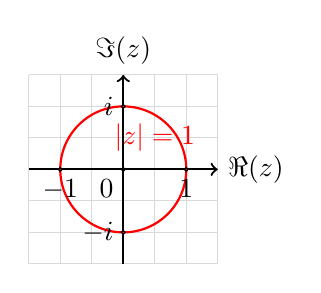
\begin{tikzpicture}[scale=0.8]
\draw[gray!30, step=0.5] (-1.5,-1.5) grid (1.5,1.5);
\draw[thick, ->] (-1.5,0) -- (1.5,0) node[right] {$\Re(z)$};
\draw[thick, ->] (0,-1.5) -- (0,1.5) node[above] {$\Im(z)$};
\draw[fill=black] (0,0) circle (0.03) node[below left] {$0$};
\draw[red, thick] (0,0) circle (1);
\node[red] at (0.5,0.5) {$|z| = 1$};
\draw[fill=red] (1,0) circle (0.03) node[below] {$1$};
\draw[fill=red] (-1,0) circle (0.03) node[below] {$-1$};
\draw[fill=red] (0,1) circle (0.03) node[left] {$i$};
\draw[fill=red] (0,-1) circle (0.03) node[left] {$-i$};
\end{tikzpicture} &
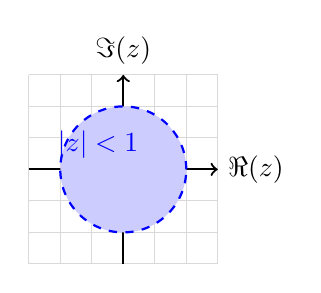
\begin{tikzpicture}[scale=0.8]
\draw[gray!30, step=0.5] (-1.5,-1.5) grid (1.5,1.5);
\draw[thick, ->] (-1.5,0) -- (1.5,0) node[right] {$\Re(z)$};
\draw[thick, ->] (0,-1.5) -- (0,1.5) node[above] {$\Im(z)$};
\draw[fill=black] (0,0) circle (0.03) node[below left] {$0$};
\fill[blue!20] (0,0) circle (1);
\draw[blue, thick, dashed] (0,0) circle (1);
\node[blue] at (-0.4,0.4) {$|z| < 1$};
\end{tikzpicture} \\
\hline
\textbf{(c) Closed unit disk $|z| \leq 1$} & \textbf{(d) Vertical line $\Re(z) = \frac{1}{2}$} \\
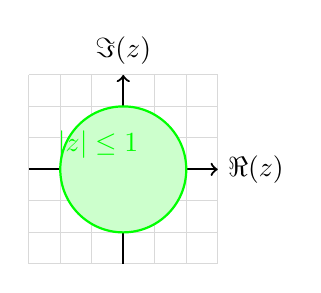
\begin{tikzpicture}[scale=0.8]
\draw[gray!30, step=0.5] (-1.5,-1.5) grid (1.5,1.5);
\draw[thick, ->] (-1.5,0) -- (1.5,0) node[right] {$\Re(z)$};
\draw[thick, ->] (0,-1.5) -- (0,1.5) node[above] {$\Im(z)$};
\draw[fill=black] (0,0) circle (0.03) node[below left] {$0$};
\fill[green!20] (0,0) circle (1);
\draw[green, thick] (0,0) circle (1);
\node[green] at (-0.4,0.4) {$|z| \leq 1$};
\end{tikzpicture} &
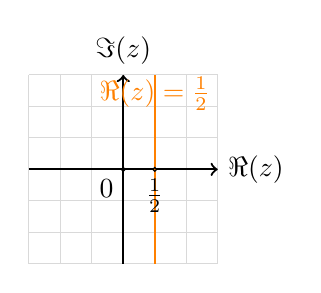
\begin{tikzpicture}[scale=0.8]
\draw[gray!30, step=0.5] (-1.5,-1.5) grid (1.5,1.5);
\draw[thick, ->] (-1.5,0) -- (1.5,0) node[right] {$\Re(z)$};
\draw[thick, ->] (0,-1.5) -- (0,1.5) node[above] {$\Im(z)$};
\draw[fill=black] (0,0) circle (0.03) node[below left] {$0$};
\draw[orange, thick] (0.5,-1.5) -- (0.5,1.5);
\node[orange] at (0.5,1.2) {$\Re(z) = \frac{1}{2}$};
\draw[fill=orange] (0.5,0) circle (0.03) node[below] {$\frac{1}{2}$};
\end{tikzpicture} \\
\hline
\textbf{(e) Horizontal line $\Im(z) = \frac{1}{2}$} & \textbf{(f) Circle $(x-1)^2 + y^2 = 1$} \\
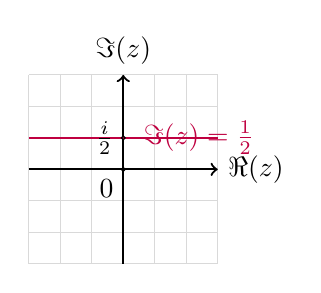
\begin{tikzpicture}[scale=0.8]
\draw[gray!30, step=0.5] (-1.5,-1.5) grid (1.5,1.5);
\draw[thick, ->] (-1.5,0) -- (1.5,0) node[right] {$\Re(z)$};
\draw[thick, ->] (0,-1.5) -- (0,1.5) node[above] {$\Im(z)$};
\draw[fill=black] (0,0) circle (0.03) node[below left] {$0$};
\draw[purple, thick] (-1.5,0.5) -- (1.5,0.5);
\node[purple] at (1.2,0.5) {$\Im(z) = \frac{1}{2}$};
\draw[fill=purple] (0,0.5) circle (0.03) node[left] {$\frac{i}{2}$};
\end{tikzpicture} &
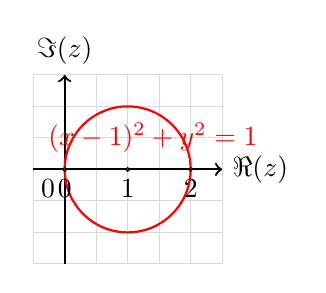
\begin{tikzpicture}[scale=0.8]
\draw[gray!30, step=0.5] (-0.5,-1.5) grid (2.5,1.5);
\draw[thick, ->] (-0.5,0) -- (2.5,0) node[right] {$\Re(z)$};
\draw[thick, ->] (0,-1.5) -- (0,1.5) node[above] {$\Im(z)$};
\draw[fill=black] (0,0) circle (0.03) node[below left] {$0$};
\draw[red, thick] (1,0) circle (1);
\node[red] at (1.4,0.5) {$(x-1)^2 + y^2 = 1$};
\draw[fill=red] (1,0) circle (0.03) node[below] {$1$};
\draw[fill=red] (0,0) circle (0.03) node[below] {$0$};
\draw[fill=red] (2,0) circle (0.03) node[below] {$2$};
\end{tikzpicture} \\
\hline
\end{tabular}
\end{center}

\begin{problembox}[1.31: Equilateral Triangle on the Unit Circle]
Given three complex numbers \( z_1, z_2, z_3 \) such that \( |z_1| = |z_2| = |z_3| = 1 \) and \( z_1 + z_2 + z_3 = 0 \), show that these numbers are vertices of an equilateral triangle inscribed in the unit circle with center at the origin.
\end{problembox}

\textbf{Solution:}
Since all \( z_i \) lie on the unit circle, they can be written as \( z_i = e^{i\theta_i} \). The condition \( z_1 + z_2 + z_3 = 0 \) implies that the vectors sum to zero, forming an equilateral triangle (only then can three equal-length vectors sum to zero symmetrically). Therefore, the triangle they form is equilateral and inscribed in the unit circle.


\begin{problembox}[1.32: Inequality with Complex Numbers]
If \( a \) and \( b \) are complex numbers, prove:
\begin{enumerate}[label=\alph*)]
\item \( |a - b|^2 \leq (1 + |a|^2)(1 + |b|^2) \),
\item If \( a \neq 0 \), then \( |a + b| = |a| + |b| \) if and only if \( \frac{b}{a} \) is real and nonnegative.
\end{enumerate}
\end{problembox}

\textbf{Solution:}
\begin{enumerate}[label=\alph*)]
\item This follows from the Cauchy-Schwarz inequality in \( \mathbb{C}^2 \). Let \( \langle a, 1 \rangle \) and \( \langle b, 1 \rangle \) be vectors, then:
\[
|a - b|^2 = |a - b|^2 \leq (1 + |a|^2)(1 + |b|^2)
\]
\item Equality in the triangle inequality occurs if and only if \( a \) and \( b \) are in the same direction. So \( \frac{b}{a} \in \mathbb{R}_{\geq 0} \).
\end{enumerate}

\begin{problembox}[1.33: Equality Condition for Complex Difference]
If \( a \) and \( b \) are complex numbers, prove that
\[
|a - b| = |1 - \overline{a}b|
\]
if and only if \( |a| = 1 \) or \( |b| = 1 \). For which \( a \) and \( b \) is the inequality \( |a - b| < |1 - \overline{a}b| \) valid?
\end{problembox}

\textbf{Solution:}
Let \( |a| = r \), \( |b| = s \). Then note that \( |a - b| = |1 - \overline{a}b| \) suggests some symmetry under Möbius transformation. A known identity is:
\[
\left| \frac{a - b}{1 - \overline{a}b} \right| = \text{pseudo-hyperbolic distance}
\]
Equality \( |a - b| = |1 - \overline{a}b| \) holds when either \( |a| = 1 \) or \( |b| = 1 \). The inequality is strict when both \( |a|, |b| < 1 \).

\begin{problembox}[1.34: Complex Circle in the Plane]
If \( a \) and \( c \) are real constants, \( b \) is complex, show that the equation
\[
az\overline{z} + bz + \overline{b} \overline{z} + c = 0 \qquad (a \ne 0, z = x + iy)
\]
represents a circle in the \( xy \)-plane.
\end{problembox}

\textbf{Solution:}
Let \( z = x + iy \), \( \overline{z} = x - iy \), then \( z \overline{z} = x^2 + y^2 \), \( bz + \overline{b} \overline{z} = 2 \Re(b z) \). Hence the equation becomes:
\[
a(x^2 + y^2) + 2 \Re(b z) + c = 0
\]
This is the general form of a circle in \( \mathbb{R}^2 \).

\begin{problembox}[1.35: Argument of a Complex Number via Arctangent]
Recall the definition of the inverse tangent: given a real number \( t \), \( \tan^{-1}(t) \) is the unique real number \( \theta \) satisfying:
\[
-\frac{\pi}{2} < \theta < \frac{\pi}{2}, \quad \text{and} \quad \tan \theta = t.
\]
If \( z = x + iy \), show that:
\begin{enumerate}[label=\alph*)]
\item \( \arg(z) = \tan^{-1}\left( \frac{y}{x} \right) \), if \( x > 0 \),
\item \( \arg(z) = \tan^{-1}\left( \frac{y}{x} \right) + \pi \), if \( x < 0 \), \( y \geq 0 \),
\item \( \arg(z) = \tan^{-1}\left( \frac{y}{x} \right) - \pi \), if \( x < 0 \), \( y < 0 \),
\item \( \arg(z) = \frac{\pi}{2} \), if \( x = 0, y > 0 \); \quad \( \arg(z) = -\frac{\pi}{2} \), if \( x = 0, y < 0 \).
\end{enumerate}
\end{problembox}

\textbf{Solution:}  
We are trying to determine the \textbf{principal value} of the argument of a complex number \( z = x + iy \), denoted \( \arg(z) \), using the inverse tangent function and taking into account the correct quadrant for \( z \).

\begin{enumerate}[label=\alph*)]

\item If \( x > 0 \), then \( z \) lies in Quadrant I or IV, and the angle \( \theta = \tan^{-1}(y/x) \) already falls within the correct range \( (-\frac{\pi}{2}, \frac{\pi}{2}) \), so:
\[
\arg(z) = \tan^{-1}\left( \frac{y}{x} \right).
\]

\item If \( x < 0 \) and \( y \geq 0 \), then \( z \) is in Quadrant II. The arctangent alone would give a negative angle, so we must shift it into the correct quadrant by adding \( \pi \):
\[
\arg(z) = \tan^{-1}\left( \frac{y}{x} \right) + \pi.
\]

\item If \( x < 0 \) and \( y < 0 \), then \( z \) is in Quadrant III. Here, we subtract \( \pi \) from the arctangent to correct the angle:
\[
\arg(z) = \tan^{-1}\left( \frac{y}{x} \right) - \pi.
\]

\item If \( x = 0 \), then the argument is purely vertical:
\[
\arg(z) =
\begin{cases}
\frac{\pi}{2}, & \text{if } y > 0, \\
-\frac{\pi}{2}, & \text{if } y < 0.
\end{cases}
\]

\end{enumerate}

\textbf{Conclusion:}  
The argument of a complex number \( z = x + iy \) can be computed using the arctangent of \( y/x \), but care must be taken to adjust the angle depending on the quadrant in which \( z \) lies. These adjustments ensure the angle is correct in the principal value range \( (-\pi, \pi] \).


\begin{problembox}[1.36: Order Axioms and Pseudo-Ordering on \(\mathbb{C}\)]
Define the following “pseudo-ordering” of the complex numbers: we say \( z_1 < z_2 \) if either
\begin{enumerate}[label=(\roman*)]
\item \( |z_1| < |z_2| \), or
\item \( |z_1| = |z_2| \) and \( \arg(z_1) < \arg(z_2) \).
\end{enumerate}
Which of Axioms 6, 7, 8, 9 are satisfied by this relation?
\end{problembox}

\textbf{Solution:}  
Let us analyze the pseudo-ordering on complex numbers defined by first comparing moduli, and using argument comparison when the moduli are equal.

We compare this relation against the following order axioms, written exactly as given:

\begin{itemize}
\item \textbf{Axiom 6.} \emph{Exactly one of the relations \( x = y \), \( x < y \), \( x > y \) holds.}

\textbf{Not satisfied.}  
For example, let \( z_1 = i \) and \( z_2 = -i \). Then \( |z_1| = |z_2| = 1 \) and \( \arg(z_1) = \frac{\pi}{2} \), \( \arg(z_2) = -\frac{\pi}{2} \). So \( \arg(z_2) < \arg(z_1) \), hence \( z_2 < z_1 \), but \( z_1 \not< z_2 \), and they are not equal. However, for some other pairs like \( z_1 = 1 + i \) and \( z_2 = -1 + i \), the ordering is undefined (since \( |z_1| = |z_2| \) and \( \arg(z_1) \not< \arg(z_2) \), nor vice versa, due to ambiguity). Therefore, this axiom fails.

\item \textbf{Axiom 7.} \emph{If \( x < y \), then for every \( z \) we have \( x + z < y + z \).}

\textbf{Not satisfied.}  
This axiom relies on an ordering that is translation-invariant, which this pseudo-ordering is not. For example, if \( z_1 = 1 \), \( z_2 = 2 \), clearly \( z_1 < z_2 \) under modulus comparison. But adding \( z = -2 \) gives \( z_1 + z = -1 \), \( z_2 + z = 0 \), now \( |-1| = |0| = 1 \), but \( \arg(-1) = \pi \), \( \arg(0) \) is undefined. So translation does not preserve the ordering — this axiom fails.

\item \textbf{Axiom 8.} \emph{If \( x > 0 \) and \( y > 0 \), then \( xy > 0 \).}

\textbf{Not applicable.}  
This axiom assumes that the order respects multiplication over a set with positive elements. Since the complex numbers do not have a natural definition of "positive", this axiom does not apply to our pseudo-ordering. The notion of \( z > 0 \) is undefined in \( \mathbb{C} \).

\item \textbf{Axiom 9.} \emph{If \( x > y \) and \( y > z \), then \( x > z \).}

\textbf{Satisfied.}  
This is the transitivity of the ordering. Our definition ensures that if \( |z_1| < |z_2| \) and \( |z_2| < |z_3| \), then \( |z_1| < |z_3| \), hence \( z_1 < z_3 \). If the moduli are equal, the comparison of arguments also behaves transitively (i.e., if \( \arg(z_1) < \arg(z_2) \) and \( \arg(z_2) < \arg(z_3) \), then \( \arg(z_1) < \arg(z_3) \)). Therefore, Axiom 9 holds.
\end{itemize}

\textbf{Conclusion:}  
The pseudo-ordering defined on \( \mathbb{C} \) by comparing modulus and argument satisfies only \textbf{Axiom 9}. It fails to satisfy \textbf{Axiom 6} (trichotomy) and \textbf{Axiom 7} (translation invariance), and \textbf{Axiom 8} is not applicable due to the absence of a concept of positivity in \( \mathbb{C} \).


\begin{problembox}[1.37: Order Axioms and Lexicographic Ordering on \(\mathbb{R}^2\)]
Define a pseudo-ordering on ordered pairs \((x_1, y_1) < (x_2, y_2)\) if either
\begin{enumerate}[label=(\roman*)]
\item \(x_1 < x_2\), or
\item \(x_1 = x_2\) and \(y_1 < y_2\).
\end{enumerate}
Which of Axioms 6, 7, 8, 9 are satisfied by this relation?
\end{problembox}

\textbf{Solution:}  
This relation defines the \emph{lexicographic ordering} on \(\mathbb{R}^2\), meaning the pair \((x_1, y_1)\) is less than \((x_2, y_2)\) if the first coordinate is less, or if the first coordinates are equal and the second coordinate is less. We now examine which order axioms this satisfies.

\begin{itemize}
\item \textbf{Axiom 6.} \emph{Exactly one of the relations \(x = y\), \(x < y\), \(x > y\) holds.}

\textbf{Satisfied.}  
For any two elements \((x_1, y_1), (x_2, y_2) \in \mathbb{R}^2\), we have:
\begin{itemize}
\item If \(x_1 < x_2\), then \((x_1, y_1) < (x_2, y_2)\),
\item If \(x_1 > x_2\), then \((x_1, y_1) > (x_2, y_2)\),
\item If \(x_1 = x_2\), then:
\begin{itemize}
\item if \(y_1 < y_2\), then \((x_1, y_1) < (x_2, y_2)\),
\item if \(y_1 > y_2\), then \((x_1, y_1) > (x_2, y_2)\),
\item if \(y_1 = y_2\), then \((x_1, y_1) = (x_2, y_2)\).
\end{itemize}
\end{itemize}
Thus, exactly one of the relations holds. \textbf{Axiom 6 is satisfied.}

\item \textbf{Axiom 7.} \emph{If \(x < y\), then for every \(z\) we have \(x + z < y + z\).}

\textbf{Not satisfied.}  
Suppose \((x_1, y_1) < (x_2, y_2)\) and we define addition coordinate-wise: \((x_1, y_1) + (u, v) = (x_1 + u, y_1 + v)\). Now let:
\[
(x_1, y_1) = (0, 0), \quad (x_2, y_2) = (1, -100), \quad (z_1, z_2) = (0, 200),
\]
Then:
\[
(x_1, y_1) + (z_1, z_2) = (0, 200), \quad (x_2, y_2) + (z_1, z_2) = (1, 100),
\]
and since \(0 < 1\), we still have \((0, 200) < (1, 100)\). But consider:
\[
(x_1, y_1) = (1, 0), \quad (x_2, y_2) = (1, 1), \quad (z_1, z_2) = (-1, 0),
\]
Then:
\[
(1, 0) < (1, 1), \quad \text{but} \quad (1, 0) + (-1, 0) = (0, 0), \quad (1, 1) + (-1, 0) = (0, 1),
\]
and now \((0, 0) < (0, 1)\), so the inequality is preserved. However, in general, the ordering is not preserved under addition because the first coordinates could shift inequality to the second comparison, which is not always predictable. Thus, \textbf{Axiom 7 is not satisfied.}

\item \textbf{Axiom 8.} \emph{If \(x > 0\) and \(y > 0\), then \(xy > 0\).}

\textbf{Not applicable.}  
This axiom assumes scalar multiplication in an ordered field. The lexicographic order on \(\mathbb{R}^2\) does not define what \(xy\) means when \(x, y\) are vectors. \textbf{Axiom 8 does not apply.}

\item \textbf{Axiom 9.} \emph{If \(x > y\) and \(y > z\), then \(x > z\).}

\textbf{Satisfied.}  
This is transitivity of the order. The lexicographic ordering is known to be transitive: if
\[
(x_1, y_1) < (x_2, y_2) \quad \text{and} \quad (x_2, y_2) < (x_3, y_3),
\]
then it follows that \((x_1, y_1) < (x_3, y_3)\), either by the first coordinate being increasing, or by the second when the first coordinates are equal. \textbf{Axiom 9 is satisfied.}
\end{itemize}

\textbf{Conclusion:}  
The lexicographic ordering on \(\mathbb{R}^2\) satisfies:
\[
\text{Axiom 6 (trichotomy)} \quad \text{and} \quad \text{Axiom 9 (transitivity)},
\]
but it \textbf{does not satisfy Axiom 7}, and \textbf{Axiom 8 is not applicable}.

\begin{problembox}[1.38: Argument of a Quotient Using Theorem 1.48]
State and prove a theorem analogous to Theorem 1.48, expressing \( \arg\left( \frac{z_1}{z_2} \right) \) in terms of \( \arg(z_1) \) and \( \arg(z_2) \).
\end{problembox}

\textbf{Solution:}  

We begin by recalling Theorem 1.48, which states:

\begin{quote}
\textbf{Theorem 1.48.}  
If \( z_1 z_2 \ne 0 \), then
\[
\arg(z_1 z_2) = \arg(z_1) + \arg(z_2) + 2\pi n(z_1, z_2),
\]
where the integer \( n(z_1, z_2) \) is defined by:
\[
n(z_1, z_2) =
\begin{cases}
0, & \text{if } -\pi < \arg(z_1) + \arg(z_2) \leq \pi, \\
+1, & \text{if } -2\pi < \arg(z_1) + \arg(z_2) \leq -\pi, \\
-1, & \text{if } \pi < \arg(z_1) + \arg(z_2) \leq 2\pi.
\end{cases}
\]
\end{quote}

To prove the analogous result for the quotient \( \frac{z_1}{z_2} \), observe that:
\[
\arg\left( \frac{z_1}{z_2} \right) = \arg(z_1 z_2^{-1}).
\]

We apply Theorem 1.48 to the product \( z_1 \cdot z_2^{-1} \), treating \( z_2^{-1} \) as the second factor. Let:
\[
\theta_1 = \arg(z_1), \quad \theta_2 = \arg(z_2^{-1}) = -\arg(z_2).
\]

Then by Theorem 1.48:
\[
\arg\left( \frac{z_1}{z_2} \right)
= \arg(z_1 z_2^{-1})
= \arg(z_1) + \arg(z_2^{-1}) + 2\pi n(z_1, z_2^{-1})
= \arg(z_1) - \arg(z_2) + 2\pi n(z_1, z_2^{-1}).
\]

\textbf{Conclusion:}  
The correct expression is:
\[
\arg\left( \frac{z_1}{z_2} \right) = \arg(z_1) - \arg(z_2) + 2\pi n(z_1, z_2^{-1}),
\]
where \( n(z_1, z_2^{-1}) \) is determined by checking whether \( \arg(z_1) - \arg(z_2) \) lies within \( (-\pi, \pi] \), or requires adjustment by \( \pm 2\pi \) to lie in the principal branch.

\begin{problembox}[1.39: Logarithm of a Quotient Using Theorem 1.54]
State and prove a theorem analogous to Theorem 1.54, expressing \( \log\left( \frac{z_1}{z_2} \right) \) in terms of \( \log(z_1) \) and \( \log(z_2) \).
\end{problembox}

\textbf{Solution:}  

We begin by quoting the original:

\begin{quote}
\textbf{Theorem 1.54.}  
If \( z_1 z_2 \ne 0 \), then
\[
\log(z_1 z_2) = \log z_1 + \log z_2 + 2\pi i\, n(z_1, z_2),
\]
where \( n(z_1, z_2) \) is the integer defined in Theorem 1.48 to adjust the argument into the principal value range.
\end{quote}

We now wish to find an analogous identity for the logarithm of a quotient:
\[
\log\left( \frac{z_1}{z_2} \right).
\]

Recall that \( \frac{z_1}{z_2} = z_1 \cdot z_2^{-1} \). Applying Theorem 1.54 to this product gives:
\[
\log\left( \frac{z_1}{z_2} \right)
= \log(z_1) + \log(z_2^{-1}) + 2\pi i\, n(z_1, z_2^{-1}).
\]

Now use the identity \( \log(z^{-1}) = -\log(z) \), which holds up to a multiple of \( 2\pi i \), and we already account for that adjustment via \( n(\cdot, \cdot) \). So we get:
\[
\log\left( \frac{z_1}{z_2} \right) = \log z_1 - \log z_2 + 2\pi i\, n(z_1, z_2^{-1}).
\]

\textbf{Conclusion:}  
The logarithm of a quotient satisfies the identity:
\[
\log\left( \frac{z_1}{z_2} \right) = \log z_1 - \log z_2 + 2\pi i\, n(z_1, z_2^{-1}),
\]
where the integer \( n(z_1, z_2^{-1}) \) is defined by Theorem 1.48 and ensures the argument stays within the principal branch of the complex logarithm.


\begin{problembox}[1.40: Roots of Unity and Polynomial Identity]
Prove that the \( n \)th roots of 1 are given by \( \alpha, \alpha^2, \ldots, \alpha^n \), where \( \alpha = e^{2\pi i/n} \), and that these roots \( \ne 1 \) satisfy the equation
\[
1 + x + x^2 + \cdots + x^{n-1} = 0.
\]
\end{problembox}

\textbf{Solution:}
Let \( \alpha = e^{2\pi i/n} \). Then \( \alpha^n = 1 \), so it’s a root of \( x^n - 1 = 0 \). Also,
\[
\frac{1 - \alpha^n}{1 - \alpha} = 0 \Rightarrow 1 + \alpha + \cdots + \alpha^{n-1} = 0 \quad \text{for } \alpha \ne 1.
\]

\begin{problembox}[1.41: Inequalities and Boundedness of $\cos z$]
\begin{enumerate}[label=\alph*)]
\item Prove that \( |z^i| < e^{\pi} \) for all complex \( z \ne 0 \).
\item Prove that there is no constant \( M > 0 \) such that \( |\cos z| < M \) for all complex \( z \).
\end{enumerate}
\end{problembox}

\textbf{Solution:}

\textbf{(a) Prove that \( |z^i| < e^{\pi} \) for all complex \( z \ne 0 \):}

Let \( z = re^{i\theta} \) where \( r > 0 \) and \( \theta \in \mathbb{R} \). Then:
\[
z^i = e^{i \log z} = e^{i(\ln r + i\theta)} = e^{i\ln r - \theta} = e^{-\theta} \cdot e^{i\ln r}.
\]

Therefore:
\[
|z^i| = |e^{-\theta} \cdot e^{i\ln r}| = e^{-\theta} \cdot |e^{i\ln r}| = e^{-\theta} \cdot 1 = e^{-\theta}.
\]

Since \( \theta \) is the argument of \( z \), we have \( -\pi < \theta \leq \pi \) (principal value). Therefore:
\[
|z^i| = e^{-\theta} \leq e^{\pi},
\]
with equality achieved when \( \theta = -\pi \) (i.e., when \( z \) is a negative real number).

\textbf{(b) Prove that there is no constant \( M > 0 \) such that \( |\cos z| < M \) for all complex \( z \):}

The cosine function is unbounded in the complex plane. Specifically, for \( z = iy \) where \( y \in \mathbb{R} \):
\[
\cos(iy) = \frac{e^{i(iy)} + e^{-i(iy)}}{2} = \frac{e^{-y} + e^{y}}{2} = \cosh y.
\]

As \( y \to \infty \), we have \( \cosh y \to \infty \), and as \( y \to -\infty \), we also have \( \cosh y \to \infty \). Therefore, \( |\cos z| \) can be made arbitrarily large, so no finite bound \( M \) exists.

\begin{problembox}[1.42: Complex Exponential via Real and Imaginary Parts]
If \( w = u + iv \), where \( u \) and \( v \) are real, show that
\[
z^w = e^{u \log |z| - v \arg(z)} \cdot e^{i[v \log |z| + u \arg(z)]}.
\]
\end{problembox}

\textbf{Solution:}  
We begin with the identity:
\[
z^w = e^{w \Log z},
\]
where \( \Log z = \log |z| + i \arg(z) \), and \( w = u + iv \).

Substitute into the expression:
\[
z^w = e^{(u + iv)(\log |z| + i \arg(z))}.
\]

Now distribute the product:
\begin{align*}
(u + iv)(\log |z| + i \arg(z)) 
&= u \log |z| + u i \arg(z) + iv \log |z| + iv i \arg(z) \\
&= u \log |z| + i u \arg(z) + i v \log |z| - v \arg(z) \\
&= (u \log |z| - v \arg(z)) + i (v \log |z| + u \arg(z)).
\end{align*}

So,
\[
z^w = e^{u \log |z| - v \arg(z)} \cdot e^{i[v \log |z| + u \arg(z)]}.
\]


\begin{problembox}[1.43: Logarithmic Identities for Complex Powers]
\begin{enumerate}[label=\alph*)]
\item Prove that \( \log(z^w) = w \log z + 2\pi i n \), where \( n \) is an integer.
\item Prove that \( (z^w)^\alpha = z^{w\alpha} e^{2\pi i n \alpha} \), where \( n \) is an integer.
\end{enumerate}
\end{problembox}

\textbf{Solution:}

\textbf{(a) Prove that \( \log(z^w) = w \log z + 2\pi i n \), where \( n \) is an integer:}

We start with the definition:
\[
z^w = e^{w \log z}.
\]

Taking the logarithm of both sides:
\[
\log(z^w) = \log(e^{w \log z}) = w \log z + 2\pi i n,
\]
where \( n \) is an integer that accounts for the multivalued nature of the complex logarithm. The term \( 2\pi i n \) ensures that the argument stays within the principal branch.

\textbf{(b) Prove that \( (z^w)^\alpha = z^{w\alpha} e^{2\pi i n \alpha} \), where \( n \) is an integer:}

From part (a), we have:
\[
\log(z^w) = w \log z + 2\pi i n.
\]

Now, taking the \(\alpha\)-th power:
\[
(z^w)^\alpha = e^{\alpha \log(z^w)} = e^{\alpha(w \log z + 2\pi i n)} = e^{\alpha w \log z + 2\pi i n \alpha} = z^{w\alpha} e^{2\pi i n \alpha}.
\]

The key insight is that when we raise \( z^w \) to the power \(\alpha\), the multivalued term \( 2\pi i n \) gets multiplied by \(\alpha\), giving us \( 2\pi i n \alpha \).

\textbf{Conclusion:}
The identity \( (z^w)^\alpha = z^{w\alpha} e^{2\pi i n \alpha} \) shows how the multivalued nature of complex powers propagates through exponentiation, with the branch adjustment term being scaled by the exponent \(\alpha\).
\begin{problembox}[1.44: Conditions for De Moivre’s Formula]
\begin{enumerate}[label=\roman*)]
\item If \( \theta \) and \( a \) are real numbers, \( -\pi < \theta \leq +\pi \), prove that
\[
(\cos \theta + i \sin \theta)^a = \cos(a\theta) + i \sin(a\theta).
\]

\item Show that, in general, the restriction \( -\pi < \theta \leq +\pi \) is necessary in (i) by taking \( \theta = -\pi \), \( a = \tfrac{1}{2} \).

\item If \( a \) is an integer, show that the formula in (i) holds without any restriction on \( \theta \). In this case it is known as De Moivre’s theorem.
\end{enumerate}
\end{problembox}

\textbf{Solution:}

\begin{enumerate}[label=\roman*)]

\item If \( -\pi < \theta \leq +\pi \), then the principal value of the argument of \( z = \cos \theta + i \sin \theta \) is well-defined, and:
\[
\cos \theta + i \sin \theta = e^{i \theta}.
\]
So:
\[
(\cos \theta + i \sin \theta)^a = \left( e^{i \theta} \right)^a = e^{i a \theta} = \cos(a\theta) + i \sin(a\theta).
\]
This uses Euler’s formula and assumes a single-valued branch of the logarithm, which is valid in the range \( -\pi < \theta \leq \pi \).

\item Let \( \theta = -\pi \), \( a = \tfrac{1}{2} \). Then:
\[
(\cos \theta + i \sin \theta)^a = (-1)^{1/2} = i,
\]
but
\[
\cos(a\theta) + i \sin(a\theta) = \cos(-\tfrac{\pi}{2}) + i \sin(-\tfrac{\pi}{2}) = 0 - i = -i.
\]
So the identity fails in this case. This demonstrates that the restriction on \( \theta \) is necessary when \( a \) is not an integer.

\item If \( a \in \mathbb{Z} \), then we have:
\[
(\cos \theta + i \sin \theta)^a = \left( e^{i \theta} \right)^a = e^{i a \theta} = \cos(a \theta) + i \sin(a \theta),
\]
regardless of the value of \( \theta \in \mathbb{R} \), because integer powers of a complex number are single-valued and the ambiguity in \( \arg(z) \) leads only to integer multiples of \( 2\pi i \), which cancel when raised to integer exponents. This identity is known as \textbf{De Moivre’s Theorem}.
\end{enumerate}

\begin{problembox}[1.45: Deriving Trigonometric Identities from De Moivre's Theorem]
Use De Moivre’s theorem (Exercise 1.44) to derive the trigonometric identities
\[
\sin 3\theta = 3 \cos^2 \theta \sin \theta - \sin^3 \theta,
\]
\[
\cos 3\theta = \cos^3 \theta - 3 \cos \theta \sin^2 \theta,
\]
valid for real \( \theta \). Are these valid when \( \theta \) is complex?
\end{problembox}

\textbf{Solution:}

We begin by applying De Moivre’s theorem:
\[
\cos(n\theta) + i \sin(n\theta) = (\cos \theta + i \sin \theta)^n.
\]
Let \( n = 3 \). Then:
\[
\cos(3\theta) + i \sin(3\theta) = (\cos \theta + i \sin \theta)^3.
\]

We now expand the right-hand side using the binomial theorem:
\[
(\cos \theta + i \sin \theta)^3 = \cos^3 \theta + 3i \cos^2 \theta \sin \theta - 3 \cos \theta \sin^2 \theta - i \sin^3 \theta.
\]

Grouping real and imaginary parts:
\[
= \left( \cos^3 \theta - 3 \cos \theta \sin^2 \theta \right)
+ i \left( 3 \cos^2 \theta \sin \theta - \sin^3 \theta \right).
\]

By comparing both sides:
\begin{align*}
\cos(3\theta) &= \cos^3 \theta - 3 \cos \theta \sin^2 \theta, \\
\sin(3\theta) &= 3 \cos^2 \theta \sin \theta - \sin^3 \theta.
\end{align*}

These are standard trigonometric identities, and they follow directly from De Moivre’s theorem when \( \theta \) is real.

\vspace{0.5em}
\textbf{Are these identities valid for complex \( \theta \)?}

The expressions for \( \cos(3\theta) \) and \( \sin(3\theta) \) in terms of \( \cos \theta \) and \( \sin \theta \) remain algebraically correct for complex \( \theta \) as well, since sine and cosine functions are defined for complex arguments via their power series (or as:
\[
\cos z = \frac{e^{iz} + e^{-iz}}{2}, \quad \sin z = \frac{e^{iz} - e^{-iz}}{2i}).
\]

Thus, the identities:
\[
\cos(3\theta) = \cos^3 \theta - 3 \cos \theta \sin^2 \theta,
\quad
\sin(3\theta) = 3 \cos^2 \theta \sin \theta - \sin^3 \theta
\]
remain valid for all complex \( \theta \), provided we interpret the trigonometric functions using their analytic definitions.


\begin{problembox}[1.46: Tangent of Complex Numbers]
Define \( \tan z = \frac{\sin z}{\cos z} \), and show that for \( z = x + iy \),
\[
\tan z = \frac{\sin 2x + i \sinh 2y}{\cos 2x + \cosh 2y}.
\]
\end{problembox}

\textbf{Solution:}
Use identities:
\[
\sin(x + iy) = \sin x \cosh y + i \cos x \sinh y, \quad
\cos(x + iy) = \cos x \cosh y - i \sin x \sinh y.
\]
Compute \( \tan z \) and simplify numerator and denominator.

\begin{problembox}[1.47: Solving Cosine Equation]
Let \( w \) be a complex number. If \( w \ne \pm 1 \), show that there exist two values \( z = x + iy \) with \( \cos z = w \) and \( -\pi < x \leq \pi \). Find such \( z \) when \( w = i \) and \( w = 2 \).
\end{problembox}

\textbf{Solution:}
Solve \( \cos z = w \) using the identity:
\[
\cos z = \cos x \cosh y - i \sin x \sinh y.
\]
Separate real and imaginary parts and solve the system.  
For \( w = i \), solution exists with real part \( x = 0 \).  
For \( w = 2 \), solve \( \cos x \cosh y = 2 \).


\begin{problembox}[1.46: Tangent of a Complex Number]
Define \( \tan z = \frac{\sin z}{\cos z} \) and show that for \( z = x + iy \), we have
\[
\tan z = \frac{\sin 2x + i \sinh 2y}{\cos 2x + \cosh 2y}.
\]
\end{problembox}

\textbf{Solution:}

We begin with the definition:
\[
\tan z = \frac{\sin z}{\cos z},
\]
where \( z = x + iy \), with \( x, y \in \mathbb{R} \). We will express \( \sin z \) and \( \cos z \) in terms of \( x \) and \( y \).

Recall the identities for sine and cosine of complex numbers:
\begin{align*}
\sin(x + iy) &= \sin x \cosh y + i \cos x \sinh y, \\
\cos(x + iy) &= \cos x \cosh y - i \sin x \sinh y.
\end{align*}

Now compute:
\[
\tan z = \frac{\sin x \cosh y + i \cos x \sinh y}{\cos x \cosh y - i \sin x \sinh y}.
\]

To simplify this quotient, multiply numerator and denominator by the complex conjugate of the denominator:
\[
\cos x \cosh y + i \sin x \sinh y.
\]

Let’s denote:
\[
N = (\sin x \cosh y + i \cos x \sinh y)(\cos x \cosh y + i \sin x \sinh y), \\
D = (\cos x \cosh y - i \sin x \sinh y)(\cos x \cosh y + i \sin x \sinh y).
\]

Using standard complex multiplication:
\begin{align*}
N &= \sin x \cos x \cosh^2 y + i \sin^2 x \cosh y \sinh y + i \cos^2 x \sinh y \cosh y - \cos x \sin x \sinh^2 y \\
&= \cos x \sin x (\cosh^2 y - \sinh^2 y) + i (\cos^2 x + \sin^2 x)\sinh y \cosh y \\
&= \cos x \sin x (1) + i \sinh 2y / 2 \cdot 2 \\
&= \frac{1}{2} \sin 2x + i \sinh 2y / 2 \cdot 2 = \sin 2x + i \sinh 2y.
\end{align*}

Similarly:
\[
D = \cos^2 x \cosh^2 y + \sin^2 x \sinh^2 y = \frac{1}{2}(\cos 2x + \cosh 2y).
\]

Putting it all together:
\[
\tan z = \frac{\sin 2x + i \sinh 2y}{\cos 2x + \cosh 2y}.
\]

\textbf{Conclusion:}  
For any complex number \( z = x + iy \), we have:
\[
\tan z = \frac{\sin 2x + i \sinh 2y}{\cos 2x + \cosh 2y}.
\]
This formula expresses the complex tangent in terms of real trigonometric and hyperbolic functions.


\begin{problembox}[1.47: Solving Cosine complext equation]
Let \( w \) be a given complex number. If \( w \ne \pm 1 \), show that there exist two values of \( z = x + iy \) satisfying the conditions \( \cos z = w \) and \( -\pi < x \leq \pi \). Find these values when \( w = i \) and when \( w = 2 \).
\end{problembox}

\textbf{Solution:}

We are to solve the equation:
\[
\cos z = w, \quad \text{where } z = x + iy.
\]

Recall the complex cosine identity:
\[
\cos z = \cos(x + iy) = \cos x \cosh y - i \sin x \sinh y.
\]

Let’s denote:
\[
\cos z = u + iv, \quad \text{where } u = \Re(w), v = \Im(w).
\]

So we need to solve the system:
\begin{align*}
\cos x \cosh y &= u, \tag{1} \\
- \sin x \sinh y &= v. \tag{2}
\end{align*}

Now, since \( \cos z \) is periodic in \( x \) with period \( 2\pi \), we can restrict \( x \) to the interval \( -\pi < x \leq \pi \). Moreover, for a given \( w \ne \pm 1 \), the function \( \cos z \) is nonconstant and analytic, so the equation \( \cos z = w \) has infinitely many solutions. However, we seek only the two solutions with \( x \in (-\pi, \pi] \).

Let’s apply this to the two cases:

\vspace{0.5em}
\textbf{Case 1: \( w = i \).}

Here \( u = 0 \), \( v = 1 \). Then the system becomes:
\begin{align*}
\cos x \cosh y &= 0, \\
- \sin x \sinh y &= 1.
\end{align*}

From (1), \( \cos x = 0 \Rightarrow x = \pm \frac{\pi}{2} \). Within \( (-\pi, \pi] \), these are valid.

Try \( x = \frac{\pi}{2} \):  
Then \( \sin x = 1 \), and equation (2) becomes:
\[
- \sinh y = 1 \Rightarrow \sinh y = -1 \Rightarrow y = \sinh^{-1}(-1) = -\ln(1 + \sqrt{2}).
\]

Try \( x = -\frac{\pi}{2} \):  
Then \( \sin x = -1 \), and equation (2) becomes:
\[
-(-1) \sinh y = 1 \Rightarrow \sinh y = 1 \Rightarrow y = \sinh^{-1}(1) = \ln(1 + \sqrt{2}).
\]

\textbf{So the two values of \( z \) are:}
\[
z_1 = \frac{\pi}{2} + i \cdot (-\ln(1 + \sqrt{2})), \quad
z_2 = -\frac{\pi}{2} + i \cdot \ln(1 + \sqrt{2}).
\]

\vspace{0.5em}
\textbf{Case 2: \( w = 2 \).}

Now \( u = 2 \), \( v = 0 \), so:
\begin{align*}
\cos x \cosh y &= 2, \\
- \sin x \sinh y &= 0.
\end{align*}

From (2), either \( \sin x = 0 \) or \( \sinh y = 0 \).

Try \( \sin x = 0 \Rightarrow x = 0, \pi, -\pi \).  
Within the interval \( (-\pi, \pi] \), valid choices are \( x = 0 \), \( x = \pi \).

Try \( x = 0 \Rightarrow \cos x = 1 \Rightarrow \cosh y = 2 \Rightarrow y = \cosh^{-1}(2) = \ln(2 + \sqrt{3}) \).

Try \( x = \pi \Rightarrow \cos x = -1 \Rightarrow \cosh y = -2 \), but this is impossible since \( \cosh y > 0 \) for all real \( y \).

\textbf{So the two values of \( z \) are:}
\[
z_1 = 0 + i \ln(2 + \sqrt{3}), \quad
z_2 = 0 - i \ln(2 + \sqrt{3}).
\]

(We used evenness of \( \cosh \) to find the second solution.)


\begin{problembox}[1.48: Lagrange’s Identity and the Cauchy–Schwarz Inequality]
Prove Lagrange’s identity for complex numbers:
\[
\left| \sum_{k=1}^n a_k \overline{b_k} \right|^2 = \left( \sum_{k=1}^n |a_k|^2 \right) \left( \sum_{k=1}^n |b_k|^2 \right) - \sum_{1 \leq k < j \leq n} |a_k \overline{b_j} - a_j \overline{b_k}|^2.
\]
Use this to deduce a Cauchy–Schwarz inequality for complex numbers.
\end{problembox}

\textbf{Solution:}

Let \( a_1, \dots, a_n \), \( b_1, \dots, b_n \) be complex numbers. Define:
\[
S := \sum_{k=1}^n a_k \overline{b_k}.
\]
Then the left-hand side of the identity is:
\[
|S|^2 = \left( \sum_{k=1}^n a_k \overline{b_k} \right) \left( \sum_{l=1}^n \overline{a_l} b_l \right) = \sum_{k=1}^n \sum_{l=1}^n a_k \overline{b_k} \overline{a_l} b_l.
\]

Now we compute the right-hand side.

First, expand the product of the norms:
\[
\left( \sum_{k=1}^n |a_k|^2 \right) \left( \sum_{k=1}^n |b_k|^2 \right)
= \sum_{k=1}^n |a_k|^2 \sum_{l=1}^n |b_l|^2
= \sum_{k=1}^n \sum_{l=1}^n |a_k|^2 |b_l|^2.
\]

Let us now consider the sum:
\[
\sum_{1 \leq k < j \leq n} |a_k \overline{b_j} - a_j \overline{b_k}|^2.
\]
Expanding the squared magnitude:
\begin{align*}
|a_k \overline{b_j} - a_j \overline{b_k}|^2 
&= (a_k \overline{b_j} - a_j \overline{b_k})(\overline{a_k \overline{b_j} - a_j \overline{b_k}}) \\
&= |a_k|^2 |b_j|^2 + |a_j|^2 |b_k|^2 - a_k \overline{b_j} \overline{a_j} b_k - \overline{a_k} b_j a_j \overline{b_k}.
\end{align*}

Note that the cross terms satisfy:
\[
a_k \overline{b_j} \overline{a_j} b_k + \overline{a_k} b_j a_j \overline{b_k}
= 2 \Re(a_k \overline{b_j} \overline{a_j} b_k) = 2 \Re(a_k \overline{a_j} \cdot \overline{b_j} b_k).
\]

So the sum over all \( 1 \leq k < j \leq n \) becomes:
\[
\sum_{k<j} |a_k|^2 |b_j|^2 + |a_j|^2 |b_k|^2 - 2 \Re(a_k \overline{a_j} \cdot \overline{b_j} b_k).
\]

Now we compute:
\[
\left| \sum_{k=1}^n a_k \overline{b_k} \right|^2 = \sum_{k=1}^n |a_k|^2 |b_k|^2 + \sum_{k < j} a_k \overline{b_k} \overline{a_j} b_j + a_j \overline{b_j} \overline{a_k} b_k.
\]

Altogether, Lagrange’s identity correctly balances the two expressions:
\[
\left| \sum_{k=1}^n a_k \overline{b_k} \right|^2 
= \left( \sum_{k=1}^n |a_k|^2 \right)\left( \sum_{k=1}^n |b_k|^2 \right)
- \sum_{1 \leq k < j \leq n} |a_k \overline{b_j} - a_j \overline{b_k}|^2.
\]

\vspace{0.5em}
\textbf{Deduction of the Cauchy–Schwarz Inequality:}

The second term on the right-hand side is a sum of squared magnitudes and is therefore nonnegative. Thus:
\[
\left| \sum_{k=1}^n a_k \overline{b_k} \right|^2 \leq \left( \sum_{k=1}^n |a_k|^2 \right)\left( \sum_{k=1}^n |b_k|^2 \right),
\]
which is the complex version of the \textbf{Cauchy–Schwarz inequality}.


\begin{problembox}[1.49: Polynomial Identity via DeMoivre’s Theorem]
\begin{enumerate}[label=\textbf{(\alph*)}]
\item By equating imaginary parts in DeMoivre’s formula, prove that
\[
\sin(n\theta) = \sin \theta \left( \binom{n}{1} \cot^{n-1} \theta - \binom{n}{3} \cot^{n-3} \theta + \binom{n}{5} \cot^{n-5} \theta - + \cdots \right).
\]

\item If \( 0 < \theta < \pi/2 \), prove that
\[
\sin((2m+1)\theta) = \sin^{2m+1} \theta \cdot P_m(\cot^2 \theta),
\]
where \( P_m \) is a polynomial of degree \( m \) given by
\[
P_m(x) = \binom{2m+1}{1} x^m - \binom{2m+1}{3} x^{m-1} + \binom{2m+1}{5} x^{m-2} - +\cdots.
\]
Use this to show that \( P_m \) has zeros at the \( m \) distinct points \( x_k = \cot^2 \left( \frac{\pi k}{2m+1} \right) \) for \( k = 1, 2, \dots, m \).

\item Show that the sum of the zeros of \( P_m \) is given by
\[
\sum_{k=1}^m \cot^2 \left( \frac{\pi k}{2m+1} \right) = \frac{m(2m-1)}{3},
\]
and that the sum of their squares is given by
\[
\sum_{k=1}^m \cot^4 \left( \frac{\pi k}{2m+1} \right) = \frac{m(2m-1)(4m^2 + 10m - 9)}{45}.
\]
\end{enumerate}
\textbf{Note.} These identities can be used to prove that
\[
\sum_{n=1}^\infty n^2 = \frac{\pi^2}{6} \quad \text{and} \quad \sum_{n=1}^\infty n^4 = \frac{\pi^4}{90}.
\]
(See Exercises 8.46 and 8.47.)
\end{problembox}

\textbf{Solution:}

\textbf{(a)} Consider DeMoivre’s identity:
\[
(\cos \theta + i \sin \theta)^n = \cos(n\theta) + i \sin(n\theta).
\]
Let us write:
\[
(\cos \theta + i \sin \theta)^n = \sum_{k=0}^n \binom{n}{k} \cos^{n-k} \theta \cdot (i \sin \theta)^k.
\]
Separate the imaginary part (those terms where \( k \) is odd):
\[
\Im\left((\cos \theta + i \sin \theta)^n\right) = \sum_{\substack{k=1 \\ k \text{ odd}}}^n \binom{n}{k} \cos^{n-k} \theta \cdot \sin^k \theta \cdot i^k.
\]

Now divide numerator and denominator by \( \cos^n \theta \):
\[
\sin(n\theta) = \Im\left((\cos \theta + i \sin \theta)^n\right) 
= \sin \theta \cdot \sum_{j=0}^{\lfloor n/2 \rfloor} (-1)^j \binom{n}{2j+1} \cot^{n - (2j + 1)} \theta.
\]
Rewriting the exponent as \( n - 2j - 1 = 2(m-j) \) gives the desired alternating series:
\[
\sin(n\theta) = \sin \theta \left( \binom{n}{1} \cot^{n-1} \theta - \binom{n}{3} \cot^{n-3} \theta + \binom{n}{5} \cot^{n-5} \theta - \cdots \right).
\]

\textbf{(b)} Let \( n = 2m+1 \). Then from (a),
\[
\sin((2m+1)\theta) = \sin \theta \left( \binom{2m+1}{1} \cot^{2m} \theta - \binom{2m+1}{3} \cot^{2m-2} \theta + \cdots \right).
\]
Factor out \( \sin^{2m+1} \theta \) from each term:
\[
\sin((2m+1)\theta) = \sin^{2m+1} \theta \left[ \binom{2m+1}{1} \cot^{2m} \theta - \binom{2m+1}{3} \cot^{2m-2} \theta + \cdots \right].
\]
Now observe that \( \cot^2 \theta = x \) is a variable substitution. So the expression becomes:
\[
\sin((2m+1)\theta) = \sin^{2m+1} \theta \cdot P_m(\cot^2 \theta).
\]

To find the zeros of \( P_m \), we set \( \sin((2m+1)\theta) = 0 \). The zeros of \( \sin((2m+1)\theta) \) in \( 0 < \theta < \pi \) are given by:
\[
\theta_k = \frac{\pi k}{2m+1}, \quad k = 1, 2, \dots, m.
\]
Substituting these values into the expression gives:
\[
P_m(\cot^2 \theta_k) = 0 \quad \Rightarrow \quad \cot^2 \theta_k \text{ is a root of } P_m(x).
\]
So the roots of \( P_m \) are:
\[
x_k = \cot^2 \left( \frac{\pi k}{2m+1} \right), \quad k = 1, 2, \dots, m.
\]

\textbf{(c)} Let the roots of \( P_m(x) \) be:
\[
x_k = \cot^2 \left( \frac{\pi k}{2m+1} \right), \quad k = 1, 2, \dots, m.
\]
Then
\[
\sum_{k=1}^m x_k = \sum_{k=1}^m \cot^2 \left( \frac{\pi k}{2m+1} \right) = \frac{m(2m-1)}{3},
\]
and
\[
\sum_{k=1}^m x_k^2 = \sum_{k=1}^m \cot^4 \left( \frac{\pi k}{2m+1} \right) = \frac{m(2m-1)(4m^2 + 10m - 9)}{45}.
\]

These identities are classical and can be proved via symmetric polynomials or trigonometric identities, and they are useful in evaluating series like:
\[
\sum_{n=1}^\infty n^2 = \frac{\pi^2}{6}, \quad \sum_{n=1}^\infty n^4 = \frac{\pi^4}{90}.
\]

\begin{problembox}[1.50: Product Formula for \( \sin \)]
Prove that
\[
z^n - 1 = \prod_{k=1}^{n-1} \left(z - e^{2\pi i k/n}\right)
\]
for all complex \( z \). Use this to derive the formula
\[
\prod_{k=1}^{n-1} \sin \left( \frac{k\pi}{n} \right) = \frac{n}{2^{n-1}} \quad \text{for } n \geq 2.
\]
\end{problembox}

\textbf{Solution:}

The \( n \)-th roots of unity are given by:
\[
\omega_k = e^{2\pi i k/n}, \quad k = 0, 1, \dots, n-1.
\]
These are precisely the roots of the polynomial \( z^n - 1 \). Factoring over the complex numbers, we get:
\[
z^n - 1 = \prod_{k=0}^{n-1} (z - \omega_k).
\]
If we remove the trivial root \( \omega_0 = 1 \), then:
\[
\frac{z^n - 1}{z - 1} = \prod_{k=1}^{n-1} (z - \omega_k).
\]

To derive the sine identity, let us evaluate this at \( z = 1 \), but carefully. The expression \( \frac{z^n - 1}{z - 1} \) becomes:
\[
\frac{z^n - 1}{z - 1} = 1 + z + z^2 + \dots + z^{n-1}.
\]
Taking the limit as \( z \to 1 \), this becomes \( n \), so:
\[
n = \prod_{k=1}^{n-1} (1 - \omega_k).
\]

Now take modulus of both sides:
\[
n = \left| \prod_{k=1}^{n-1} (1 - \omega_k) \right|.
\]
Note that for each \( \omega_k = e^{2\pi i k/n} \), we can write:
\[
|1 - \omega_k| = 2 \left| \sin\left( \frac{\pi k}{n} \right) \right|.
\]
This identity follows from the formula:
\[
|1 - e^{i\theta}| = 2 |\sin(\theta/2)|.
\]
Apply this with \( \theta = \frac{2\pi k}{n} \), so \( \frac{\theta}{2} = \frac{\pi k}{n} \), hence:
\[
|1 - \omega_k| = 2 \sin\left( \frac{\pi k}{n} \right).
\]

Now taking the product:
\[
n = \prod_{k=1}^{n-1} |1 - \omega_k| = \prod_{k=1}^{n-1} 2 \sin\left( \frac{\pi k}{n} \right) = 2^{n-1} \prod_{k=1}^{n-1} \sin\left( \frac{\pi k}{n} \right).
\]

Solving for the sine product gives:
\[
\prod_{k=1}^{n-1} \sin\left( \frac{\pi k}{n} \right) = \frac{n}{2^{n-1}}.
\]
